\documentclass[twoside]{book}

% Packages required by doxygen
\usepackage{fixltx2e}
\usepackage{calc}
\usepackage{doxygen}
\usepackage[export]{adjustbox} % also loads graphicx
\usepackage{graphicx}
\usepackage[utf8]{inputenc}
\usepackage{makeidx}
\usepackage{multicol}
\usepackage{multirow}
\PassOptionsToPackage{warn}{textcomp}
\usepackage{textcomp}
\usepackage[nointegrals]{wasysym}
\usepackage[table]{xcolor}

% Font selection
\usepackage[T1]{fontenc}
\usepackage[scaled=.90]{helvet}
\usepackage{courier}
\usepackage{amssymb}
\usepackage{sectsty}
\renewcommand{\familydefault}{\sfdefault}
\allsectionsfont{%
  \fontseries{bc}\selectfont%
  \color{darkgray}%
}
\renewcommand{\DoxyLabelFont}{%
  \fontseries{bc}\selectfont%
  \color{darkgray}%
}
\newcommand{\+}{\discretionary{\mbox{\scriptsize$\hookleftarrow$}}{}{}}

% Page & text layout
\usepackage{geometry}
\geometry{%
  a4paper,%
  top=2.5cm,%
  bottom=2.5cm,%
  left=2.5cm,%
  right=2.5cm%
}
\tolerance=750
\hfuzz=15pt
\hbadness=750
\setlength{\emergencystretch}{15pt}
\setlength{\parindent}{0cm}
\setlength{\parskip}{3ex plus 2ex minus 2ex}
\makeatletter
\renewcommand{\paragraph}{%
  \@startsection{paragraph}{4}{0ex}{-1.0ex}{1.0ex}{%
    \normalfont\normalsize\bfseries\SS@parafont%
  }%
}
\renewcommand{\subparagraph}{%
  \@startsection{subparagraph}{5}{0ex}{-1.0ex}{1.0ex}{%
    \normalfont\normalsize\bfseries\SS@subparafont%
  }%
}
\makeatother

% Headers & footers
\usepackage{fancyhdr}
\pagestyle{fancyplain}
\fancyhead[LE]{\fancyplain{}{\bfseries\thepage}}
\fancyhead[CE]{\fancyplain{}{}}
\fancyhead[RE]{\fancyplain{}{\bfseries\leftmark}}
\fancyhead[LO]{\fancyplain{}{\bfseries\rightmark}}
\fancyhead[CO]{\fancyplain{}{}}
\fancyhead[RO]{\fancyplain{}{\bfseries\thepage}}
\fancyfoot[LE]{\fancyplain{}{}}
\fancyfoot[CE]{\fancyplain{}{}}
\fancyfoot[RE]{\fancyplain{}{\bfseries\scriptsize Generated by Doxygen }}
\fancyfoot[LO]{\fancyplain{}{\bfseries\scriptsize Generated by Doxygen }}
\fancyfoot[CO]{\fancyplain{}{}}
\fancyfoot[RO]{\fancyplain{}{}}
\renewcommand{\footrulewidth}{0.4pt}
\renewcommand{\chaptermark}[1]{%
  \markboth{#1}{}%
}
\renewcommand{\sectionmark}[1]{%
  \markright{\thesection\ #1}%
}

% Indices & bibliography
\usepackage{natbib}
\usepackage[titles]{tocloft}
\setcounter{tocdepth}{3}
\setcounter{secnumdepth}{5}
\makeindex

% Hyperlinks (required, but should be loaded last)
\usepackage{ifpdf}
\ifpdf
  \usepackage[pdftex,pagebackref=true]{hyperref}
\else
  \usepackage[ps2pdf,pagebackref=true]{hyperref}
\fi
\hypersetup{%
  colorlinks=true,%
  linkcolor=blue,%
  citecolor=blue,%
  unicode%
}

% Custom commands
\newcommand{\clearemptydoublepage}{%
  \newpage{\pagestyle{empty}\cleardoublepage}%
}

\usepackage{caption}
\captionsetup{labelsep=space,justification=centering,font={bf},singlelinecheck=off,skip=4pt,position=top}

%===== C O N T E N T S =====

\begin{document}

% Titlepage & ToC
\hypersetup{pageanchor=false,
             bookmarksnumbered=true,
             pdfencoding=unicode
            }
\pagenumbering{roman}
\begin{titlepage}
\vspace*{7cm}
\begin{center}%
{\Large My Project }\\
\vspace*{1cm}
{\large Generated by Doxygen 1.8.11}\\
\end{center}
\end{titlepage}
\clearemptydoublepage
\tableofcontents
\clearemptydoublepage
\pagenumbering{arabic}
\hypersetup{pageanchor=true}

%--- Begin generated contents ---
\chapter{Hierarchical Index}
\section{Class Hierarchy}
This inheritance list is sorted roughly, but not completely, alphabetically\+:\begin{DoxyCompactList}
\item \contentsline{section}{Result\+Pair}{\pageref{classResultPair}}{}
\item Serializable\begin{DoxyCompactList}
\item \contentsline{section}{Domain\+Validator}{\pageref{classDomainValidator}}{}
\item \contentsline{section}{Inet\+Address\+Validator}{\pageref{classInetAddressValidator}}{}
\item \contentsline{section}{Regex\+Validator}{\pageref{classRegexValidator}}{}
\item \contentsline{section}{Url\+Validator}{\pageref{classUrlValidator}}{}
\end{DoxyCompactList}
\item Test\+Case\begin{DoxyCompactList}
\item \contentsline{section}{Url\+Validator\+Test}{\pageref{classUrlValidatorTest}}{}
\end{DoxyCompactList}
\end{DoxyCompactList}

\chapter{Data Structure Index}
\section{Data Structures}
Here are the data structures with brief descriptions\+:\begin{DoxyCompactList}
\item\contentsline{section}{\hyperlink{structgameState}{game\+State} }{\pageref{structgameState}}{}
\end{DoxyCompactList}

\chapter{Data Structure Documentation}
\hypertarget{classDomainValidator}{}\section{Domain\+Validator Class Reference}
\label{classDomainValidator}\index{Domain\+Validator@{Domain\+Validator}}


Inheritance diagram for Domain\+Validator\+:\nopagebreak
\begin{figure}[H]
\begin{center}
\leavevmode
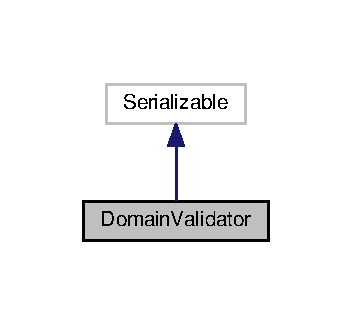
\includegraphics[width=169pt]{classDomainValidator__inherit__graph}
\end{center}
\end{figure}


Collaboration diagram for Domain\+Validator\+:\nopagebreak
\begin{figure}[H]
\begin{center}
\leavevmode
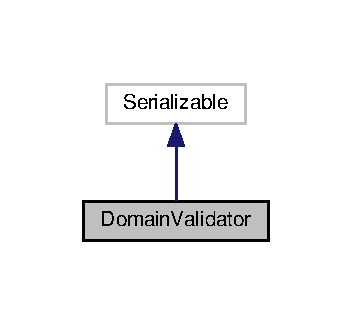
\includegraphics[width=169pt]{classDomainValidator__coll__graph}
\end{center}
\end{figure}
\subsection*{Public Member Functions}
\begin{DoxyCompactItemize}
\item 
boolean \hyperlink{classDomainValidator_a73165784191fb2f12c0bd5295b8e6004}{is\+Valid} (String domain)
\item 
boolean \hyperlink{classDomainValidator_aa05e0803e9f7390577f072fbeac0afb6}{is\+Valid\+Tld} (String tld)
\item 
boolean \hyperlink{classDomainValidator_acf198e86d538d0c001020ee8ff117b78}{is\+Valid\+Infrastructure\+Tld} (String i\+Tld)
\item 
boolean \hyperlink{classDomainValidator_a4d8d33106c0f174b9402cf78687644a5}{is\+Valid\+Generic\+Tld} (String g\+Tld)
\item 
boolean \hyperlink{classDomainValidator_ada2c219d4cec8346ebefc981a17c6bb9}{is\+Valid\+Country\+Code\+Tld} (String cc\+Tld)
\item 
boolean \hyperlink{classDomainValidator_a504c7f2f180d6cf946e2fe08915f9a88}{is\+Valid\+Local\+Tld} (String i\+Tld)
\end{DoxyCompactItemize}
\subsection*{Static Public Member Functions}
\begin{DoxyCompactItemize}
\item 
static \hyperlink{classDomainValidator}{Domain\+Validator} \hyperlink{classDomainValidator_abfe4cdfd8653602ecfc36c3b38e2dbf8}{get\+Instance} ()
\item 
static \hyperlink{classDomainValidator}{Domain\+Validator} \hyperlink{classDomainValidator_ab2f892047c9988557afbd36b3d4031bf}{get\+Instance} (boolean allow\+Local)
\end{DoxyCompactItemize}


\subsection{Detailed Description}
{\bfseries Domain name} validation routines.

This validator provides methods for validating Internet domain names and top-\/level domains. 

Domain names are evaluated according to the standards \href{http://www.ietf.org/rfc/rfc1034.txt}{\tt R\+F\+C1034}, section 3, and \href{http://www.ietf.org/rfc/rfc1123.txt}{\tt R\+F\+C1123}, section 2.\+1. No accomodation is provided for the specialized needs of other applications; if the domain name has been U\+R\+L-\/encoded, for example, validation will fail even though the equivalent plaintext version of the same name would have passed. 

Validation is also provided for top-\/level domains (T\+L\+Ds) as defined and maintained by the Internet Assigned Numbers Authority (I\+A\+NA)\+: 


\begin{DoxyItemize}
\item \hyperlink{classDomainValidator_acf198e86d538d0c001020ee8ff117b78}{is\+Valid\+Infrastructure\+Tld} -\/ validates infrastructure T\+L\+Ds ({\ttfamily .arpa}, etc.) 
\item \hyperlink{classDomainValidator_a4d8d33106c0f174b9402cf78687644a5}{is\+Valid\+Generic\+Tld} -\/ validates generic T\+L\+Ds ({\ttfamily .com, .org}, etc.) 
\item \hyperlink{classDomainValidator_ada2c219d4cec8346ebefc981a17c6bb9}{is\+Valid\+Country\+Code\+Tld} -\/ validates country code T\+L\+Ds ({\ttfamily .us, .uk, .cn}, etc.) 
\end{DoxyItemize}

({\bfseries N\+O\+TE}\+: This class does not provide IP address lookup for domain names or methods to ensure that a given domain name matches a specific IP; see \hyperlink{}{java.\+net.\+Inet\+Address} for that functionality.) 

\begin{DoxyVersion}{Version}

\end{DoxyVersion}
\begin{DoxyParagraph}{Revision}
1227719 
\end{DoxyParagraph}
\begin{DoxyParagraph}{Date}
2012-\/01-\/05 09\+:45\+:51 -\/0800 (Thu, 05 Jan 2012) 
\end{DoxyParagraph}
\begin{DoxySince}{Since}
Validator 1.\+4 
\end{DoxySince}


\subsection{Member Function Documentation}
\index{Domain\+Validator@{Domain\+Validator}!get\+Instance@{get\+Instance}}
\index{get\+Instance@{get\+Instance}!Domain\+Validator@{Domain\+Validator}}
\subsubsection[{\texorpdfstring{get\+Instance()}{getInstance()}}]{\setlength{\rightskip}{0pt plus 5cm}static {\bf Domain\+Validator} Domain\+Validator.\+get\+Instance (
\begin{DoxyParamCaption}
{}
\end{DoxyParamCaption}
)\hspace{0.3cm}{\ttfamily [static]}}\hypertarget{classDomainValidator_abfe4cdfd8653602ecfc36c3b38e2dbf8}{}\label{classDomainValidator_abfe4cdfd8653602ecfc36c3b38e2dbf8}
Returns the singleton instance of this validator. It will not consider local addresses as valid. \begin{DoxyReturn}{Returns}
the singleton instance of this validator 
\end{DoxyReturn}


Here is the caller graph for this function\+:
\nopagebreak
\begin{figure}[H]
\begin{center}
\leavevmode
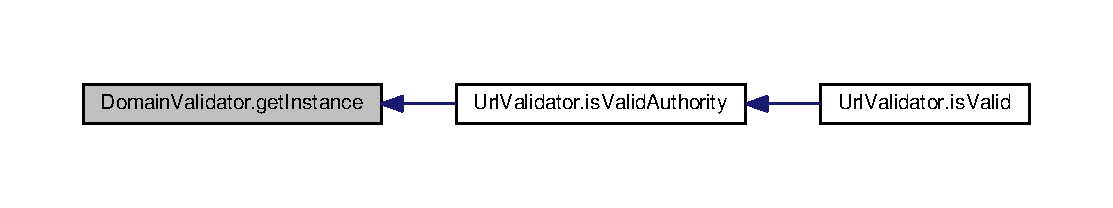
\includegraphics[width=350pt]{classDomainValidator_abfe4cdfd8653602ecfc36c3b38e2dbf8_icgraph}
\end{center}
\end{figure}


\index{Domain\+Validator@{Domain\+Validator}!get\+Instance@{get\+Instance}}
\index{get\+Instance@{get\+Instance}!Domain\+Validator@{Domain\+Validator}}
\subsubsection[{\texorpdfstring{get\+Instance(boolean allow\+Local)}{getInstance(boolean allowLocal)}}]{\setlength{\rightskip}{0pt plus 5cm}static {\bf Domain\+Validator} Domain\+Validator.\+get\+Instance (
\begin{DoxyParamCaption}
\item[{boolean}]{allow\+Local}
\end{DoxyParamCaption}
)\hspace{0.3cm}{\ttfamily [static]}}\hypertarget{classDomainValidator_ab2f892047c9988557afbd36b3d4031bf}{}\label{classDomainValidator_ab2f892047c9988557afbd36b3d4031bf}
Returns the singleton instance of this validator, with local validation as required. 
\begin{DoxyParams}{Parameters}
{\em allow\+Local} & Should local addresses be considered valid? \\
\hline
\end{DoxyParams}
\begin{DoxyReturn}{Returns}
the singleton instance of this validator 
\end{DoxyReturn}
\index{Domain\+Validator@{Domain\+Validator}!is\+Valid@{is\+Valid}}
\index{is\+Valid@{is\+Valid}!Domain\+Validator@{Domain\+Validator}}
\subsubsection[{\texorpdfstring{is\+Valid(\+String domain)}{isValid(String domain)}}]{\setlength{\rightskip}{0pt plus 5cm}boolean Domain\+Validator.\+is\+Valid (
\begin{DoxyParamCaption}
\item[{String}]{domain}
\end{DoxyParamCaption}
)}\hypertarget{classDomainValidator_a73165784191fb2f12c0bd5295b8e6004}{}\label{classDomainValidator_a73165784191fb2f12c0bd5295b8e6004}
Returns true if the specified {\ttfamily String} parses as a valid domain name with a recognized top-\/level domain. The parsing is case-\/sensitive. 
\begin{DoxyParams}{Parameters}
{\em domain} & the parameter to check for domain name syntax \\
\hline
\end{DoxyParams}
\begin{DoxyReturn}{Returns}
true if the parameter is a valid domain name 
\end{DoxyReturn}


Here is the call graph for this function\+:\nopagebreak
\begin{figure}[H]
\begin{center}
\leavevmode
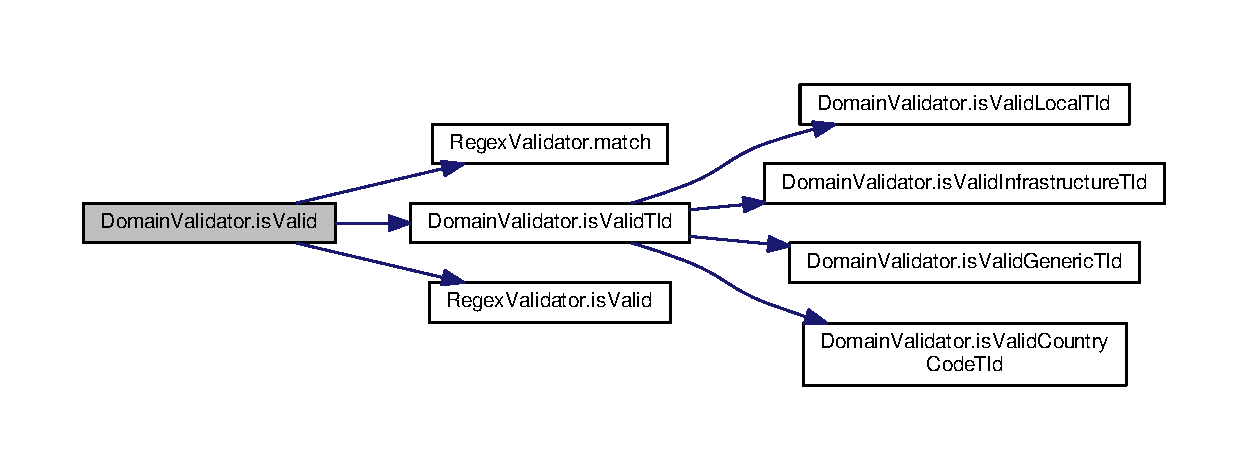
\includegraphics[width=350pt]{classDomainValidator_a73165784191fb2f12c0bd5295b8e6004_cgraph}
\end{center}
\end{figure}




Here is the caller graph for this function\+:
\nopagebreak
\begin{figure}[H]
\begin{center}
\leavevmode
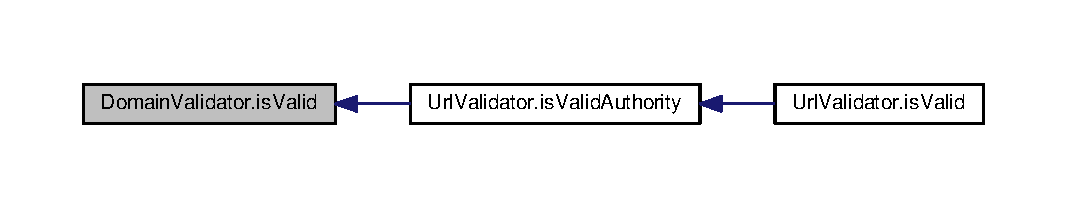
\includegraphics[width=350pt]{classDomainValidator_a73165784191fb2f12c0bd5295b8e6004_icgraph}
\end{center}
\end{figure}


\index{Domain\+Validator@{Domain\+Validator}!is\+Valid\+Country\+Code\+Tld@{is\+Valid\+Country\+Code\+Tld}}
\index{is\+Valid\+Country\+Code\+Tld@{is\+Valid\+Country\+Code\+Tld}!Domain\+Validator@{Domain\+Validator}}
\subsubsection[{\texorpdfstring{is\+Valid\+Country\+Code\+Tld(\+String cc\+Tld)}{isValidCountryCodeTld(String ccTld)}}]{\setlength{\rightskip}{0pt plus 5cm}boolean Domain\+Validator.\+is\+Valid\+Country\+Code\+Tld (
\begin{DoxyParamCaption}
\item[{String}]{cc\+Tld}
\end{DoxyParamCaption}
)}\hypertarget{classDomainValidator_ada2c219d4cec8346ebefc981a17c6bb9}{}\label{classDomainValidator_ada2c219d4cec8346ebefc981a17c6bb9}
Returns true if the specified {\ttfamily String} matches any I\+A\+N\+A-\/defined country code top-\/level domain. Leading dots are ignored if present. The search is case-\/sensitive. 
\begin{DoxyParams}{Parameters}
{\em cc\+Tld} & the parameter to check for country code T\+LD status \\
\hline
\end{DoxyParams}
\begin{DoxyReturn}{Returns}
true if the parameter is a country code T\+LD 
\end{DoxyReturn}


Here is the caller graph for this function\+:
\nopagebreak
\begin{figure}[H]
\begin{center}
\leavevmode
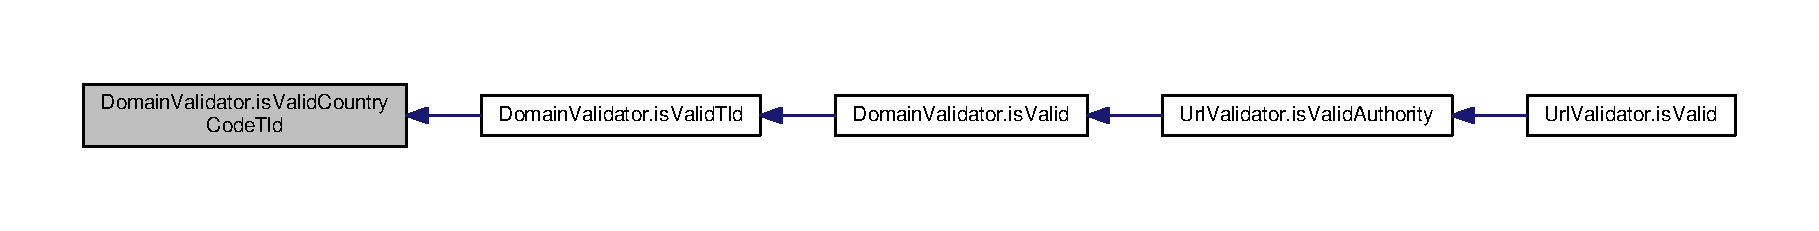
\includegraphics[width=350pt]{classDomainValidator_ada2c219d4cec8346ebefc981a17c6bb9_icgraph}
\end{center}
\end{figure}


\index{Domain\+Validator@{Domain\+Validator}!is\+Valid\+Generic\+Tld@{is\+Valid\+Generic\+Tld}}
\index{is\+Valid\+Generic\+Tld@{is\+Valid\+Generic\+Tld}!Domain\+Validator@{Domain\+Validator}}
\subsubsection[{\texorpdfstring{is\+Valid\+Generic\+Tld(\+String g\+Tld)}{isValidGenericTld(String gTld)}}]{\setlength{\rightskip}{0pt plus 5cm}boolean Domain\+Validator.\+is\+Valid\+Generic\+Tld (
\begin{DoxyParamCaption}
\item[{String}]{g\+Tld}
\end{DoxyParamCaption}
)}\hypertarget{classDomainValidator_a4d8d33106c0f174b9402cf78687644a5}{}\label{classDomainValidator_a4d8d33106c0f174b9402cf78687644a5}
Returns true if the specified {\ttfamily String} matches any I\+A\+N\+A-\/defined generic top-\/level domain. Leading dots are ignored if present. The search is case-\/sensitive. 
\begin{DoxyParams}{Parameters}
{\em g\+Tld} & the parameter to check for generic T\+LD status \\
\hline
\end{DoxyParams}
\begin{DoxyReturn}{Returns}
true if the parameter is a generic T\+LD 
\end{DoxyReturn}


Here is the caller graph for this function\+:
\nopagebreak
\begin{figure}[H]
\begin{center}
\leavevmode
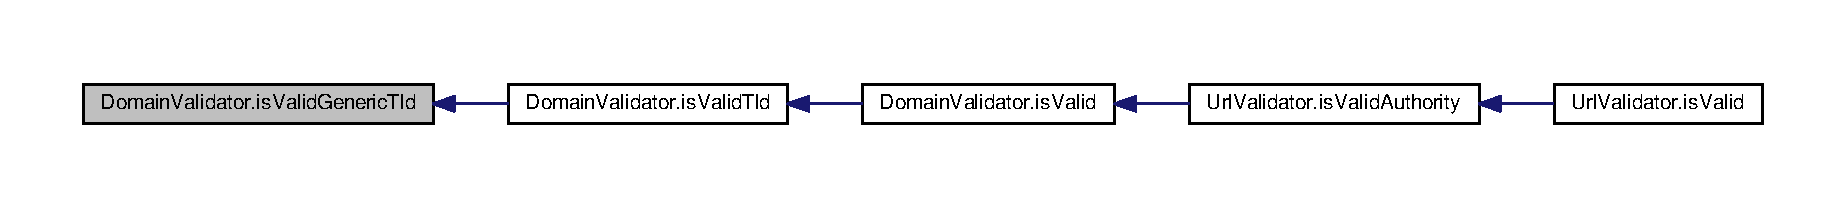
\includegraphics[width=350pt]{classDomainValidator_a4d8d33106c0f174b9402cf78687644a5_icgraph}
\end{center}
\end{figure}


\index{Domain\+Validator@{Domain\+Validator}!is\+Valid\+Infrastructure\+Tld@{is\+Valid\+Infrastructure\+Tld}}
\index{is\+Valid\+Infrastructure\+Tld@{is\+Valid\+Infrastructure\+Tld}!Domain\+Validator@{Domain\+Validator}}
\subsubsection[{\texorpdfstring{is\+Valid\+Infrastructure\+Tld(\+String i\+Tld)}{isValidInfrastructureTld(String iTld)}}]{\setlength{\rightskip}{0pt plus 5cm}boolean Domain\+Validator.\+is\+Valid\+Infrastructure\+Tld (
\begin{DoxyParamCaption}
\item[{String}]{i\+Tld}
\end{DoxyParamCaption}
)}\hypertarget{classDomainValidator_acf198e86d538d0c001020ee8ff117b78}{}\label{classDomainValidator_acf198e86d538d0c001020ee8ff117b78}
Returns true if the specified {\ttfamily String} matches any I\+A\+N\+A-\/defined infrastructure top-\/level domain. Leading dots are ignored if present. The search is case-\/sensitive. 
\begin{DoxyParams}{Parameters}
{\em i\+Tld} & the parameter to check for infrastructure T\+LD status \\
\hline
\end{DoxyParams}
\begin{DoxyReturn}{Returns}
true if the parameter is an infrastructure T\+LD 
\end{DoxyReturn}


Here is the caller graph for this function\+:
\nopagebreak
\begin{figure}[H]
\begin{center}
\leavevmode
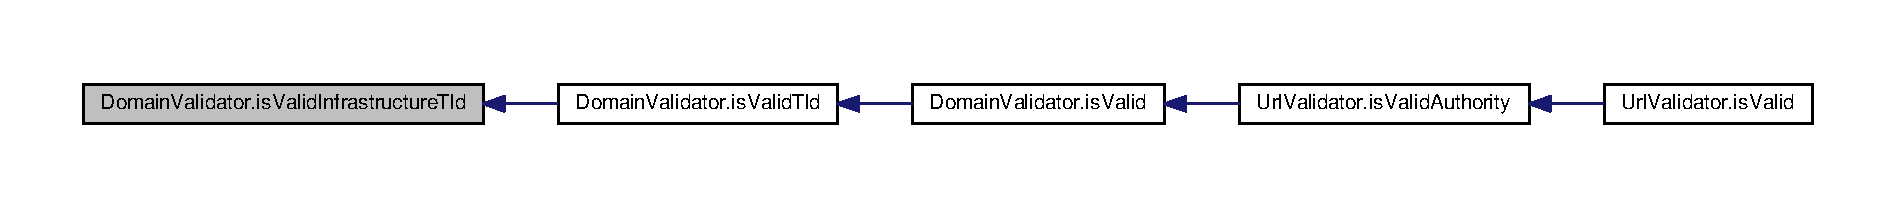
\includegraphics[width=350pt]{classDomainValidator_acf198e86d538d0c001020ee8ff117b78_icgraph}
\end{center}
\end{figure}


\index{Domain\+Validator@{Domain\+Validator}!is\+Valid\+Local\+Tld@{is\+Valid\+Local\+Tld}}
\index{is\+Valid\+Local\+Tld@{is\+Valid\+Local\+Tld}!Domain\+Validator@{Domain\+Validator}}
\subsubsection[{\texorpdfstring{is\+Valid\+Local\+Tld(\+String i\+Tld)}{isValidLocalTld(String iTld)}}]{\setlength{\rightskip}{0pt plus 5cm}boolean Domain\+Validator.\+is\+Valid\+Local\+Tld (
\begin{DoxyParamCaption}
\item[{String}]{i\+Tld}
\end{DoxyParamCaption}
)}\hypertarget{classDomainValidator_a504c7f2f180d6cf946e2fe08915f9a88}{}\label{classDomainValidator_a504c7f2f180d6cf946e2fe08915f9a88}
Returns true if the specified {\ttfamily String} matches any widely used \char`\"{}local\char`\"{} domains (localhost or localdomain). Leading dots are ignored if present. The search is case-\/sensitive. 
\begin{DoxyParams}{Parameters}
{\em i\+Tld} & the parameter to check for local T\+LD status \\
\hline
\end{DoxyParams}
\begin{DoxyReturn}{Returns}
true if the parameter is an local T\+LD 
\end{DoxyReturn}


Here is the caller graph for this function\+:
\nopagebreak
\begin{figure}[H]
\begin{center}
\leavevmode
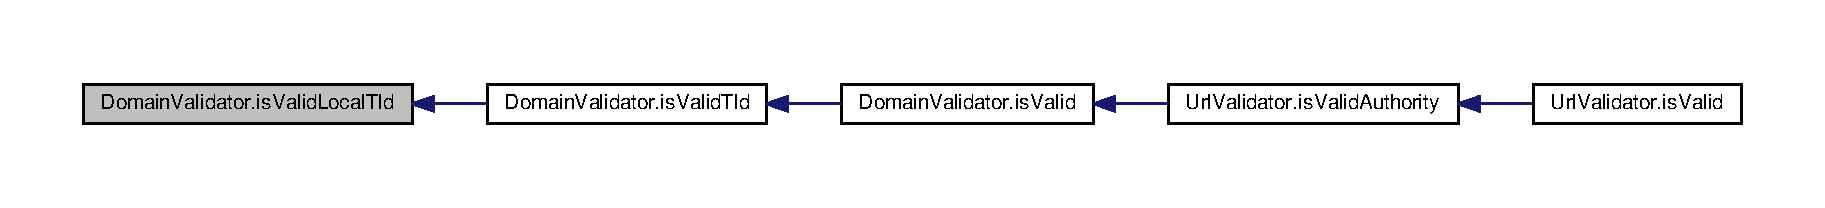
\includegraphics[width=350pt]{classDomainValidator_a504c7f2f180d6cf946e2fe08915f9a88_icgraph}
\end{center}
\end{figure}


\index{Domain\+Validator@{Domain\+Validator}!is\+Valid\+Tld@{is\+Valid\+Tld}}
\index{is\+Valid\+Tld@{is\+Valid\+Tld}!Domain\+Validator@{Domain\+Validator}}
\subsubsection[{\texorpdfstring{is\+Valid\+Tld(\+String tld)}{isValidTld(String tld)}}]{\setlength{\rightskip}{0pt plus 5cm}boolean Domain\+Validator.\+is\+Valid\+Tld (
\begin{DoxyParamCaption}
\item[{String}]{tld}
\end{DoxyParamCaption}
)}\hypertarget{classDomainValidator_aa05e0803e9f7390577f072fbeac0afb6}{}\label{classDomainValidator_aa05e0803e9f7390577f072fbeac0afb6}
Returns true if the specified {\ttfamily String} matches any I\+A\+N\+A-\/defined top-\/level domain. Leading dots are ignored if present. The search is case-\/sensitive. 
\begin{DoxyParams}{Parameters}
{\em tld} & the parameter to check for T\+LD status \\
\hline
\end{DoxyParams}
\begin{DoxyReturn}{Returns}
true if the parameter is a T\+LD 
\end{DoxyReturn}


Here is the call graph for this function\+:\nopagebreak
\begin{figure}[H]
\begin{center}
\leavevmode
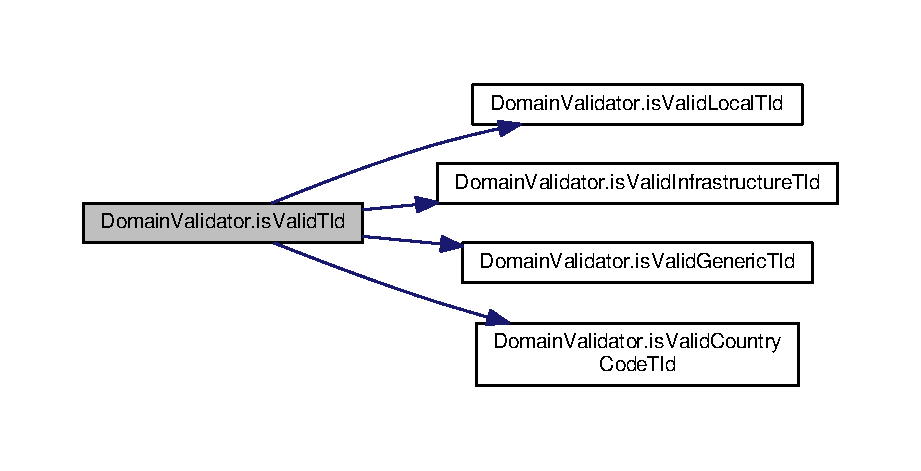
\includegraphics[width=350pt]{classDomainValidator_aa05e0803e9f7390577f072fbeac0afb6_cgraph}
\end{center}
\end{figure}




Here is the caller graph for this function\+:
\nopagebreak
\begin{figure}[H]
\begin{center}
\leavevmode
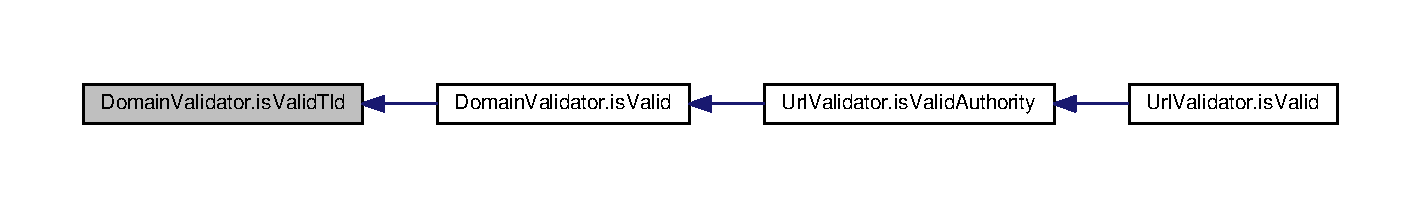
\includegraphics[width=350pt]{classDomainValidator_aa05e0803e9f7390577f072fbeac0afb6_icgraph}
\end{center}
\end{figure}




The documentation for this class was generated from the following file\+:\begin{DoxyCompactItemize}
\item 
src/Domain\+Validator.\+java\end{DoxyCompactItemize}

\hypertarget{classInetAddressValidator}{}\section{Inet\+Address\+Validator Class Reference}
\label{classInetAddressValidator}\index{Inet\+Address\+Validator@{Inet\+Address\+Validator}}


Inheritance diagram for Inet\+Address\+Validator\+:
\nopagebreak
\begin{figure}[H]
\begin{center}
\leavevmode
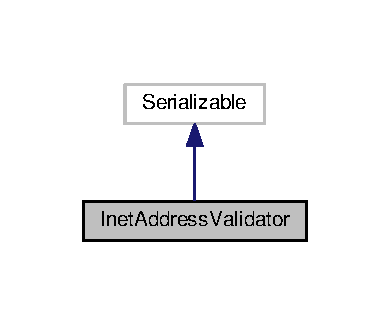
\includegraphics[width=187pt]{classInetAddressValidator__inherit__graph}
\end{center}
\end{figure}


Collaboration diagram for Inet\+Address\+Validator\+:
\nopagebreak
\begin{figure}[H]
\begin{center}
\leavevmode
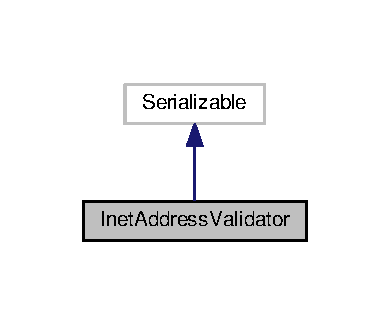
\includegraphics[width=187pt]{classInetAddressValidator__coll__graph}
\end{center}
\end{figure}
\subsection*{Public Member Functions}
\begin{DoxyCompactItemize}
\item 
boolean \hyperlink{classInetAddressValidator_a266ab1d773ca178093917c9c2faae01a}{is\+Valid} (String inet\+Address)
\item 
boolean \hyperlink{classInetAddressValidator_a2bbbd69ca6baf133c01da93a5ad1b600}{is\+Valid\+Inet4\+Address} (String inet4\+Address)
\end{DoxyCompactItemize}
\subsection*{Static Public Member Functions}
\begin{DoxyCompactItemize}
\item 
static \hyperlink{classInetAddressValidator}{Inet\+Address\+Validator} \hyperlink{classInetAddressValidator_ab9dc7787b620b11cd97b860b3ec942af}{get\+Instance} ()
\end{DoxyCompactItemize}


\subsection{Detailed Description}
{\bfseries Inet\+Address} validation and conversion routines ({\ttfamily java.\+net.\+Inet\+Address}).

This class provides methods to validate a candidate IP address.

This class is a Singleton; you can retrieve the instance via the \hyperlink{classInetAddressValidator_ab9dc7787b620b11cd97b860b3ec942af}{get\+Instance()} method. 

\begin{DoxyVersion}{Version}

\end{DoxyVersion}
\begin{DoxyParagraph}{Revision}
1227719 
\end{DoxyParagraph}
\begin{DoxySince}{Since}
Validator 1.\+4 
\end{DoxySince}


\subsection{Member Function Documentation}
\index{Inet\+Address\+Validator@{Inet\+Address\+Validator}!get\+Instance@{get\+Instance}}
\index{get\+Instance@{get\+Instance}!Inet\+Address\+Validator@{Inet\+Address\+Validator}}
\subsubsection[{\texorpdfstring{get\+Instance()}{getInstance()}}]{\setlength{\rightskip}{0pt plus 5cm}static {\bf Inet\+Address\+Validator} Inet\+Address\+Validator.\+get\+Instance (
\begin{DoxyParamCaption}
{}
\end{DoxyParamCaption}
)\hspace{0.3cm}{\ttfamily [inline]}, {\ttfamily [static]}}\hypertarget{classInetAddressValidator_ab9dc7787b620b11cd97b860b3ec942af}{}\label{classInetAddressValidator_ab9dc7787b620b11cd97b860b3ec942af}
Returns the singleton instance of this validator. \begin{DoxyReturn}{Returns}
the singleton instance of this validator 
\end{DoxyReturn}


Here is the caller graph for this function\+:
\nopagebreak
\begin{figure}[H]
\begin{center}
\leavevmode
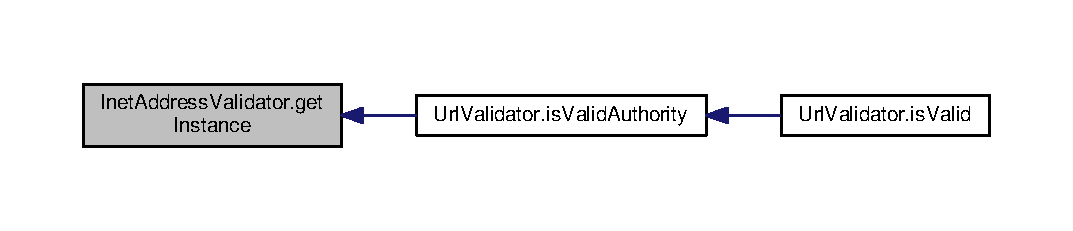
\includegraphics[width=350pt]{classInetAddressValidator_ab9dc7787b620b11cd97b860b3ec942af_icgraph}
\end{center}
\end{figure}


\index{Inet\+Address\+Validator@{Inet\+Address\+Validator}!is\+Valid@{is\+Valid}}
\index{is\+Valid@{is\+Valid}!Inet\+Address\+Validator@{Inet\+Address\+Validator}}
\subsubsection[{\texorpdfstring{is\+Valid(\+String inet\+Address)}{isValid(String inetAddress)}}]{\setlength{\rightskip}{0pt plus 5cm}boolean Inet\+Address\+Validator.\+is\+Valid (
\begin{DoxyParamCaption}
\item[{String}]{inet\+Address}
\end{DoxyParamCaption}
)\hspace{0.3cm}{\ttfamily [inline]}}\hypertarget{classInetAddressValidator_a266ab1d773ca178093917c9c2faae01a}{}\label{classInetAddressValidator_a266ab1d773ca178093917c9c2faae01a}
Checks if the specified string is a valid IP address. 
\begin{DoxyParams}{Parameters}
{\em inet\+Address} & the string to validate \\
\hline
\end{DoxyParams}
\begin{DoxyReturn}{Returns}
true if the string validates as an IP address 
\end{DoxyReturn}


Here is the call graph for this function\+:
\nopagebreak
\begin{figure}[H]
\begin{center}
\leavevmode
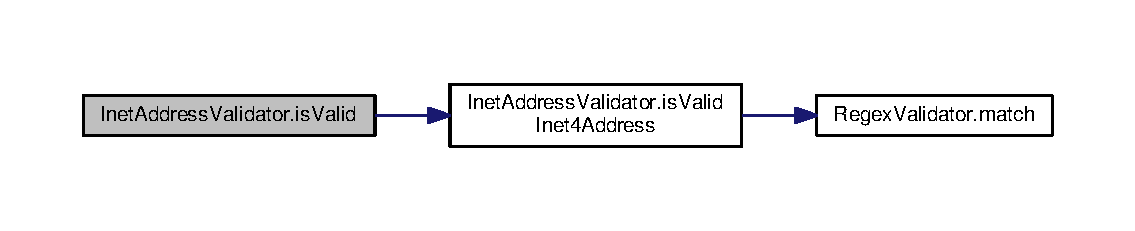
\includegraphics[width=350pt]{classInetAddressValidator_a266ab1d773ca178093917c9c2faae01a_cgraph}
\end{center}
\end{figure}




Here is the caller graph for this function\+:
\nopagebreak
\begin{figure}[H]
\begin{center}
\leavevmode
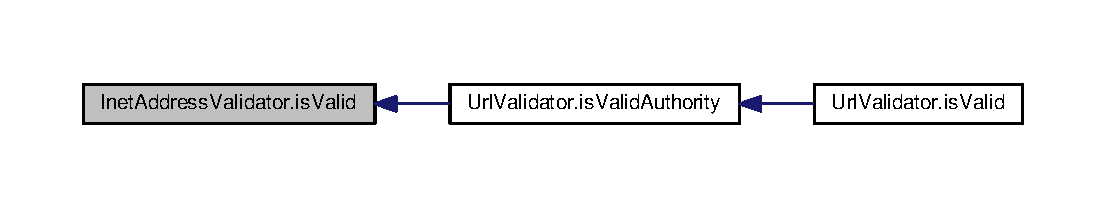
\includegraphics[width=350pt]{classInetAddressValidator_a266ab1d773ca178093917c9c2faae01a_icgraph}
\end{center}
\end{figure}


\index{Inet\+Address\+Validator@{Inet\+Address\+Validator}!is\+Valid\+Inet4\+Address@{is\+Valid\+Inet4\+Address}}
\index{is\+Valid\+Inet4\+Address@{is\+Valid\+Inet4\+Address}!Inet\+Address\+Validator@{Inet\+Address\+Validator}}
\subsubsection[{\texorpdfstring{is\+Valid\+Inet4\+Address(\+String inet4\+Address)}{isValidInet4Address(String inet4Address)}}]{\setlength{\rightskip}{0pt plus 5cm}boolean Inet\+Address\+Validator.\+is\+Valid\+Inet4\+Address (
\begin{DoxyParamCaption}
\item[{String}]{inet4\+Address}
\end{DoxyParamCaption}
)\hspace{0.3cm}{\ttfamily [inline]}}\hypertarget{classInetAddressValidator_a2bbbd69ca6baf133c01da93a5ad1b600}{}\label{classInetAddressValidator_a2bbbd69ca6baf133c01da93a5ad1b600}
Validates an I\+Pv4 address. Returns true if valid. 
\begin{DoxyParams}{Parameters}
{\em inet4\+Address} & the I\+Pv4 address to validate \\
\hline
\end{DoxyParams}
\begin{DoxyReturn}{Returns}
true if the argument contains a valid I\+Pv4 address 
\end{DoxyReturn}


Here is the call graph for this function\+:
\nopagebreak
\begin{figure}[H]
\begin{center}
\leavevmode
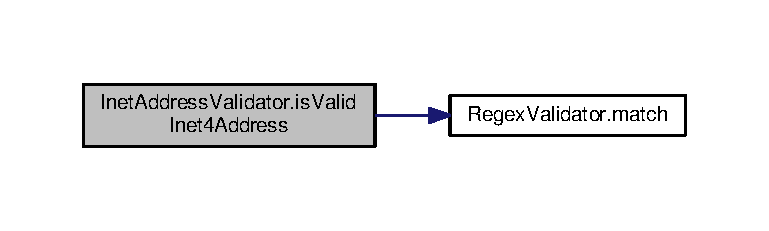
\includegraphics[width=350pt]{classInetAddressValidator_a2bbbd69ca6baf133c01da93a5ad1b600_cgraph}
\end{center}
\end{figure}




Here is the caller graph for this function\+:
\nopagebreak
\begin{figure}[H]
\begin{center}
\leavevmode
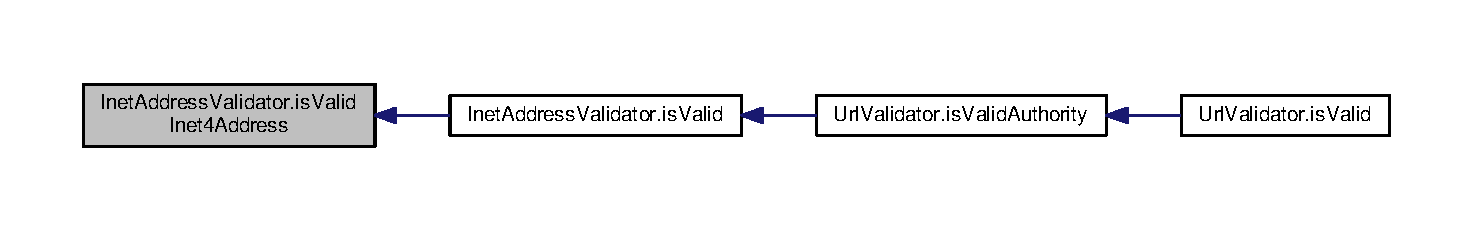
\includegraphics[width=350pt]{classInetAddressValidator_a2bbbd69ca6baf133c01da93a5ad1b600_icgraph}
\end{center}
\end{figure}




The documentation for this class was generated from the following file\+:\begin{DoxyCompactItemize}
\item 
src/Inet\+Address\+Validator.\+java\end{DoxyCompactItemize}

\hypertarget{classRegexValidator}{}\section{Regex\+Validator Class Reference}
\label{classRegexValidator}\index{Regex\+Validator@{Regex\+Validator}}


Inheritance diagram for Regex\+Validator\+:
\nopagebreak
\begin{figure}[H]
\begin{center}
\leavevmode
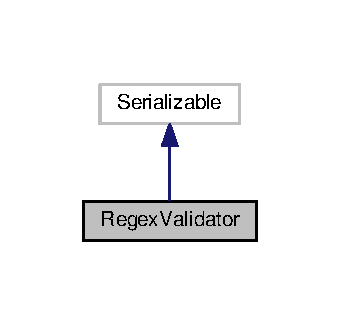
\includegraphics[width=163pt]{classRegexValidator__inherit__graph}
\end{center}
\end{figure}


Collaboration diagram for Regex\+Validator\+:
\nopagebreak
\begin{figure}[H]
\begin{center}
\leavevmode
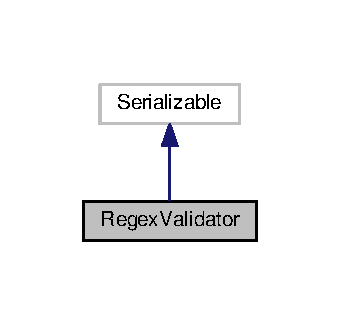
\includegraphics[width=163pt]{classRegexValidator__coll__graph}
\end{center}
\end{figure}
\subsection*{Public Member Functions}
\begin{DoxyCompactItemize}
\item 
\hyperlink{classRegexValidator_a6aebddf94f8fcd8e3e59c5f815fe91d9}{Regex\+Validator} (String regex)
\item 
\hyperlink{classRegexValidator_a58c7266d66ccd96f86427b2f3b05ca36}{Regex\+Validator} (String regex, boolean case\+Sensitive)
\item 
\hyperlink{classRegexValidator_a71a78f0ac0a7d799dcb3b769659fe1f6}{Regex\+Validator} (String\mbox{[}$\,$\mbox{]} regexs)
\item 
\hyperlink{classRegexValidator_acc8868d903890615c99044b841a79265}{Regex\+Validator} (String\mbox{[}$\,$\mbox{]} regexs, boolean case\+Sensitive)
\item 
boolean \hyperlink{classRegexValidator_adf161a2df40e7d80be0088a20af715d2}{is\+Valid} (String value)
\item 
String\mbox{[}$\,$\mbox{]} \hyperlink{classRegexValidator_aa4c1660ff32c1aecc8f616a2cfef80ed}{match} (String value)
\item 
String \hyperlink{classRegexValidator_a4ded906679cf17678ba42604b90c9e86}{validate} (String value)
\item 
String \hyperlink{classRegexValidator_a504dcfb95f1458ff9fa479404a50090e}{to\+String} ()
\end{DoxyCompactItemize}


\subsection{Detailed Description}
{\bfseries Regular Expression} validation (using J\+DK 1.\+4+ regex support). 

Construct the validator either for a single regular expression or a set (array) of regular expressions. By default validation is {\itshape case sensitive} but constructors are provided to allow {\itshape case in-\/sensitive} validation. For example to create a validator which does {\itshape case in-\/sensitive} validation for a set of regular expressions\+: 
\begin{DoxyPre}
        String[] regexs = new String[] \{...\};
        \hyperlink{classRegexValidator}{RegexValidator} validator = new \hyperlink{classRegexValidator}{RegexValidator(regexs, false)};
\end{DoxyPre}
 


\begin{DoxyItemize}
\item Validate {\ttfamily true} or {\ttfamily false}\+: 
\begin{DoxyItemize}
\item {\ttfamily boolean valid = validator.\+is\+Valid(value);} 
\end{DoxyItemize}
\item Validate returning an aggregated String of the matched groups\+: 
\begin{DoxyItemize}
\item {\ttfamily String result = validator.\+validate(value);} 
\end{DoxyItemize}
\item Validate returning the matched groups\+: 
\begin{DoxyItemize}
\item {\ttfamily String\mbox{[}\mbox{]} result = validator.\+match(value);} 
\end{DoxyItemize}
\end{DoxyItemize}

Cached instances pre-\/compile and re-\/use \hyperlink{}{Pattern}(s) -\/ which according to the \hyperlink{}{Pattern} A\+PI are safe to use in a multi-\/threaded environment.

\begin{DoxyVersion}{Version}

\end{DoxyVersion}
\begin{DoxyParagraph}{Revision}
1227719 
\end{DoxyParagraph}
\begin{DoxyParagraph}{Date}
2012-\/01-\/05 09\+:45\+:51 -\/0800 (Thu, 05 Jan 2012) 
\end{DoxyParagraph}
\begin{DoxySince}{Since}
Validator 1.\+4 
\end{DoxySince}


\subsection{Constructor \& Destructor Documentation}
\index{Regex\+Validator@{Regex\+Validator}!Regex\+Validator@{Regex\+Validator}}
\index{Regex\+Validator@{Regex\+Validator}!Regex\+Validator@{Regex\+Validator}}
\subsubsection[{\texorpdfstring{Regex\+Validator(\+String regex)}{RegexValidator(String regex)}}]{\setlength{\rightskip}{0pt plus 5cm}Regex\+Validator.\+Regex\+Validator (
\begin{DoxyParamCaption}
\item[{String}]{regex}
\end{DoxyParamCaption}
)\hspace{0.3cm}{\ttfamily [inline]}}\hypertarget{classRegexValidator_a6aebddf94f8fcd8e3e59c5f815fe91d9}{}\label{classRegexValidator_a6aebddf94f8fcd8e3e59c5f815fe91d9}
Construct a {\itshape case sensitive} validator for a single regular expression.


\begin{DoxyParams}{Parameters}
{\em regex} & The regular expression this validator will validate against \\
\hline
\end{DoxyParams}
\index{Regex\+Validator@{Regex\+Validator}!Regex\+Validator@{Regex\+Validator}}
\index{Regex\+Validator@{Regex\+Validator}!Regex\+Validator@{Regex\+Validator}}
\subsubsection[{\texorpdfstring{Regex\+Validator(\+String regex, boolean case\+Sensitive)}{RegexValidator(String regex, boolean caseSensitive)}}]{\setlength{\rightskip}{0pt plus 5cm}Regex\+Validator.\+Regex\+Validator (
\begin{DoxyParamCaption}
\item[{String}]{regex, }
\item[{boolean}]{case\+Sensitive}
\end{DoxyParamCaption}
)\hspace{0.3cm}{\ttfamily [inline]}}\hypertarget{classRegexValidator_a58c7266d66ccd96f86427b2f3b05ca36}{}\label{classRegexValidator_a58c7266d66ccd96f86427b2f3b05ca36}
Construct a validator for a single regular expression with the specified case sensitivity.


\begin{DoxyParams}{Parameters}
{\em regex} & The regular expression this validator will validate against \\
\hline
{\em case\+Sensitive} & when {\ttfamily true} matching is {\itshape case sensitive}, otherwise matching is {\itshape case in-\/sensitive} \\
\hline
\end{DoxyParams}
\index{Regex\+Validator@{Regex\+Validator}!Regex\+Validator@{Regex\+Validator}}
\index{Regex\+Validator@{Regex\+Validator}!Regex\+Validator@{Regex\+Validator}}
\subsubsection[{\texorpdfstring{Regex\+Validator(\+String[] regexs)}{RegexValidator(String[] regexs)}}]{\setlength{\rightskip}{0pt plus 5cm}Regex\+Validator.\+Regex\+Validator (
\begin{DoxyParamCaption}
\item[{String\mbox{[}$\,$\mbox{]}}]{regexs}
\end{DoxyParamCaption}
)\hspace{0.3cm}{\ttfamily [inline]}}\hypertarget{classRegexValidator_a71a78f0ac0a7d799dcb3b769659fe1f6}{}\label{classRegexValidator_a71a78f0ac0a7d799dcb3b769659fe1f6}
Construct a {\itshape case sensitive} validator that matches any one of the set of regular expressions.


\begin{DoxyParams}{Parameters}
{\em regexs} & The set of regular expressions this validator will validate against \\
\hline
\end{DoxyParams}
\index{Regex\+Validator@{Regex\+Validator}!Regex\+Validator@{Regex\+Validator}}
\index{Regex\+Validator@{Regex\+Validator}!Regex\+Validator@{Regex\+Validator}}
\subsubsection[{\texorpdfstring{Regex\+Validator(\+String[] regexs, boolean case\+Sensitive)}{RegexValidator(String[] regexs, boolean caseSensitive)}}]{\setlength{\rightskip}{0pt plus 5cm}Regex\+Validator.\+Regex\+Validator (
\begin{DoxyParamCaption}
\item[{String\mbox{[}$\,$\mbox{]}}]{regexs, }
\item[{boolean}]{case\+Sensitive}
\end{DoxyParamCaption}
)\hspace{0.3cm}{\ttfamily [inline]}}\hypertarget{classRegexValidator_acc8868d903890615c99044b841a79265}{}\label{classRegexValidator_acc8868d903890615c99044b841a79265}
Construct a validator that matches any one of the set of regular expressions with the specified case sensitivity.


\begin{DoxyParams}{Parameters}
{\em regexs} & The set of regular expressions this validator will validate against \\
\hline
{\em case\+Sensitive} & when {\ttfamily true} matching is {\itshape case sensitive}, otherwise matching is {\itshape case in-\/sensitive} \\
\hline
\end{DoxyParams}


\subsection{Member Function Documentation}
\index{Regex\+Validator@{Regex\+Validator}!is\+Valid@{is\+Valid}}
\index{is\+Valid@{is\+Valid}!Regex\+Validator@{Regex\+Validator}}
\subsubsection[{\texorpdfstring{is\+Valid(\+String value)}{isValid(String value)}}]{\setlength{\rightskip}{0pt plus 5cm}boolean Regex\+Validator.\+is\+Valid (
\begin{DoxyParamCaption}
\item[{String}]{value}
\end{DoxyParamCaption}
)\hspace{0.3cm}{\ttfamily [inline]}}\hypertarget{classRegexValidator_adf161a2df40e7d80be0088a20af715d2}{}\label{classRegexValidator_adf161a2df40e7d80be0088a20af715d2}
Validate a value against the set of regular expressions.


\begin{DoxyParams}{Parameters}
{\em value} & The value to validate. \\
\hline
\end{DoxyParams}
\begin{DoxyReturn}{Returns}
{\ttfamily true} if the value is valid otherwise {\ttfamily false}. 
\end{DoxyReturn}


Here is the caller graph for this function\+:
\nopagebreak
\begin{figure}[H]
\begin{center}
\leavevmode
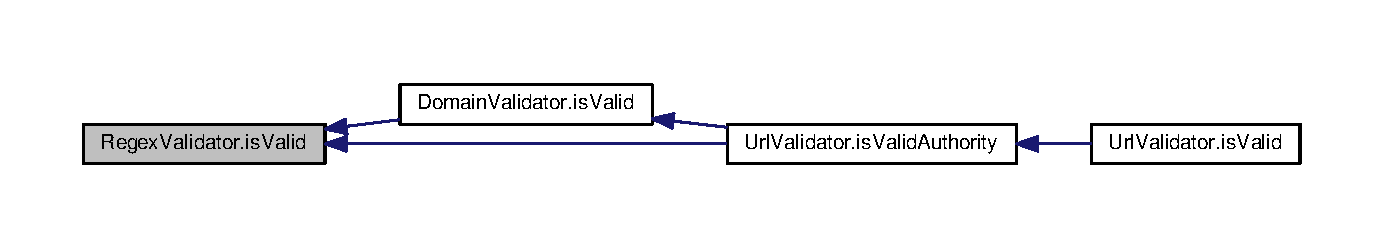
\includegraphics[width=350pt]{classRegexValidator_adf161a2df40e7d80be0088a20af715d2_icgraph}
\end{center}
\end{figure}


\index{Regex\+Validator@{Regex\+Validator}!match@{match}}
\index{match@{match}!Regex\+Validator@{Regex\+Validator}}
\subsubsection[{\texorpdfstring{match(\+String value)}{match(String value)}}]{\setlength{\rightskip}{0pt plus 5cm}String \mbox{[}$\,$\mbox{]} Regex\+Validator.\+match (
\begin{DoxyParamCaption}
\item[{String}]{value}
\end{DoxyParamCaption}
)\hspace{0.3cm}{\ttfamily [inline]}}\hypertarget{classRegexValidator_aa4c1660ff32c1aecc8f616a2cfef80ed}{}\label{classRegexValidator_aa4c1660ff32c1aecc8f616a2cfef80ed}
Validate a value against the set of regular expressions returning the array of matched groups.


\begin{DoxyParams}{Parameters}
{\em value} & The value to validate. \\
\hline
\end{DoxyParams}
\begin{DoxyReturn}{Returns}
String array of the {\itshape groups} matched if valid or {\ttfamily null} if invalid 
\end{DoxyReturn}


Here is the caller graph for this function\+:
\nopagebreak
\begin{figure}[H]
\begin{center}
\leavevmode
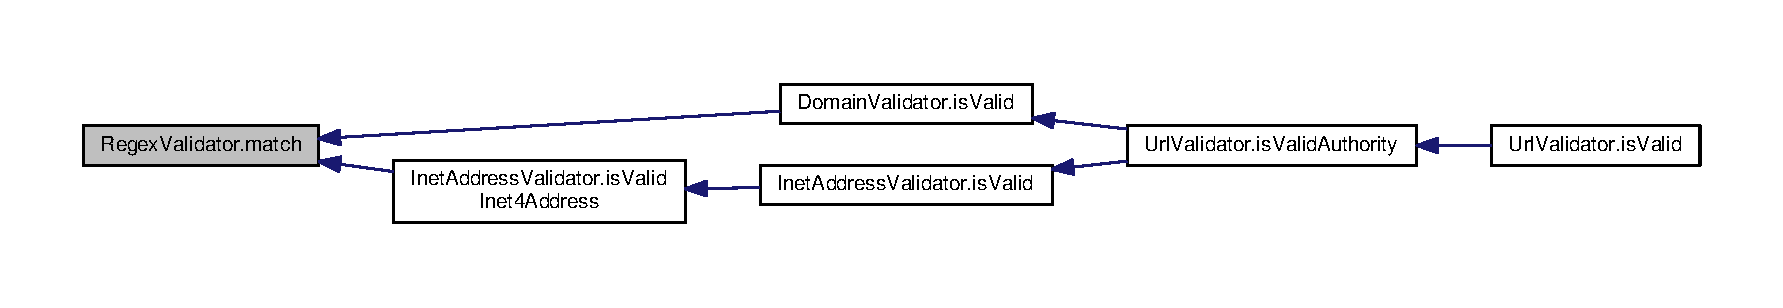
\includegraphics[width=350pt]{classRegexValidator_aa4c1660ff32c1aecc8f616a2cfef80ed_icgraph}
\end{center}
\end{figure}


\index{Regex\+Validator@{Regex\+Validator}!to\+String@{to\+String}}
\index{to\+String@{to\+String}!Regex\+Validator@{Regex\+Validator}}
\subsubsection[{\texorpdfstring{to\+String()}{toString()}}]{\setlength{\rightskip}{0pt plus 5cm}String Regex\+Validator.\+to\+String (
\begin{DoxyParamCaption}
{}
\end{DoxyParamCaption}
)\hspace{0.3cm}{\ttfamily [inline]}}\hypertarget{classRegexValidator_a504dcfb95f1458ff9fa479404a50090e}{}\label{classRegexValidator_a504dcfb95f1458ff9fa479404a50090e}
Provide a String representation of this validator. \begin{DoxyReturn}{Returns}
A String representation of this validator 
\end{DoxyReturn}
\index{Regex\+Validator@{Regex\+Validator}!validate@{validate}}
\index{validate@{validate}!Regex\+Validator@{Regex\+Validator}}
\subsubsection[{\texorpdfstring{validate(\+String value)}{validate(String value)}}]{\setlength{\rightskip}{0pt plus 5cm}String Regex\+Validator.\+validate (
\begin{DoxyParamCaption}
\item[{String}]{value}
\end{DoxyParamCaption}
)\hspace{0.3cm}{\ttfamily [inline]}}\hypertarget{classRegexValidator_a4ded906679cf17678ba42604b90c9e86}{}\label{classRegexValidator_a4ded906679cf17678ba42604b90c9e86}
Validate a value against the set of regular expressions returning a String value of the aggregated groups.


\begin{DoxyParams}{Parameters}
{\em value} & The value to validate. \\
\hline
\end{DoxyParams}
\begin{DoxyReturn}{Returns}
Aggregated String value comprised of the {\itshape groups} matched if valid or {\ttfamily null} if invalid 
\end{DoxyReturn}


The documentation for this class was generated from the following file\+:\begin{DoxyCompactItemize}
\item 
src/Regex\+Validator.\+java\end{DoxyCompactItemize}

\hypertarget{classResultPair}{}\section{Result\+Pair Class Reference}
\label{classResultPair}\index{Result\+Pair@{Result\+Pair}}
\subsection*{Public Member Functions}
\begin{DoxyCompactItemize}
\item 
{\bfseries Result\+Pair} (String item, boolean valid)\hypertarget{classResultPair_a68f95e8177e171c52276175c9cfd4496}{}\label{classResultPair_a68f95e8177e171c52276175c9cfd4496}

\end{DoxyCompactItemize}
\subsection*{Data Fields}
\begin{DoxyCompactItemize}
\item 
String {\bfseries item}\hypertarget{classResultPair_a57f116b1233276d56ac8a725e9b8ee74}{}\label{classResultPair_a57f116b1233276d56ac8a725e9b8ee74}

\item 
boolean {\bfseries valid}\hypertarget{classResultPair_a219ec2c717341670988da0bce0b34fae}{}\label{classResultPair_a219ec2c717341670988da0bce0b34fae}

\end{DoxyCompactItemize}


\subsection{Detailed Description}
Groups tests and expected results.

\begin{DoxyVersion}{Version}

\end{DoxyVersion}
\begin{DoxyParagraph}{Revision}
588091 
\end{DoxyParagraph}
\begin{DoxyParagraph}{Date}
2007-\/10-\/24 17\+:17\+:42 -\/0700 (Wed, 24 Oct 2007) 
\end{DoxyParagraph}


The documentation for this class was generated from the following file\+:\begin{DoxyCompactItemize}
\item 
src/Result\+Pair.\+java\end{DoxyCompactItemize}

\hypertarget{classUrlValidator}{}\section{Url\+Validator Class Reference}
\label{classUrlValidator}\index{Url\+Validator@{Url\+Validator}}


Inheritance diagram for Url\+Validator\+:\nopagebreak
\begin{figure}[H]
\begin{center}
\leavevmode
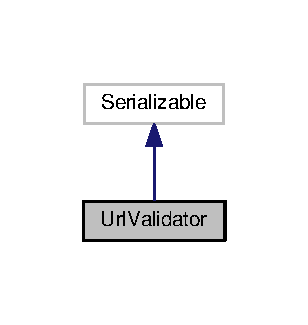
\includegraphics[width=148pt]{classUrlValidator__inherit__graph}
\end{center}
\end{figure}


Collaboration diagram for Url\+Validator\+:\nopagebreak
\begin{figure}[H]
\begin{center}
\leavevmode
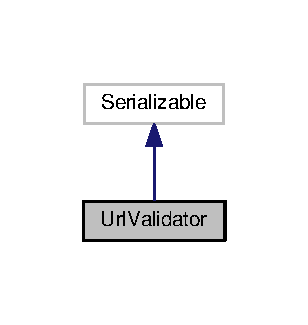
\includegraphics[width=148pt]{classUrlValidator__coll__graph}
\end{center}
\end{figure}
\subsection*{Public Member Functions}
\begin{DoxyCompactItemize}
\item 
\hyperlink{classUrlValidator_aca1390e63674c0a23797c7cc06a30564}{Url\+Validator} ()
\item 
\hyperlink{classUrlValidator_acb49224c5b8936840f734120586ea09d}{Url\+Validator} (String\mbox{[}$\,$\mbox{]} schemes)
\item 
\hyperlink{classUrlValidator_ab4c272f9342b7a3e4b4184ee18a1d45e}{Url\+Validator} (long options)
\item 
\hyperlink{classUrlValidator_aaea06225017e4030284d1f487f530798}{Url\+Validator} (String\mbox{[}$\,$\mbox{]} schemes, long options)
\item 
\hyperlink{classUrlValidator_a4dcb6938b73df2c093739f03ac6ed52d}{Url\+Validator} (\hyperlink{classRegexValidator}{Regex\+Validator} authority\+Validator, long options)
\item 
\hyperlink{classUrlValidator_ae6e7b13ef1b296d2220239213c4c50b1}{Url\+Validator} (String\mbox{[}$\,$\mbox{]} schemes, \hyperlink{classRegexValidator}{Regex\+Validator} authority\+Validator, long options)
\item 
boolean \hyperlink{classUrlValidator_aad892796e16502238af06e5de73f1325}{is\+Valid} (String value)
\end{DoxyCompactItemize}
\subsection*{Static Public Member Functions}
\begin{DoxyCompactItemize}
\item 
static \hyperlink{classUrlValidator}{Url\+Validator} \hyperlink{classUrlValidator_aeb644e3bf40f37b798b450f15421bfad}{get\+Instance} ()
\end{DoxyCompactItemize}
\subsection*{Static Public Attributes}
\begin{DoxyCompactItemize}
\item 
static final long \hyperlink{classUrlValidator_a1cd6766c458c99db9d98b585417a9623}{A\+L\+L\+O\+W\+\_\+\+A\+L\+L\+\_\+\+S\+C\+H\+E\+M\+ES} = 1 $<$$<$ 0
\item 
static final long \hyperlink{classUrlValidator_a2a0966f94123825fcef6816a5d684ed2}{A\+L\+L\+O\+W\+\_\+2\+\_\+\+S\+L\+A\+S\+H\+ES} = 1 $<$$<$ 1
\item 
static final long \hyperlink{classUrlValidator_a9f6b028f570818955c807cfe97e29641}{N\+O\+\_\+\+F\+R\+A\+G\+M\+E\+N\+TS} = 1 $<$$<$ 2
\item 
static final long \hyperlink{classUrlValidator_a8614b7832fddf98bff7ddfb5dfdbff75}{A\+L\+L\+O\+W\+\_\+\+L\+O\+C\+A\+L\+\_\+\+U\+R\+LS} = 1 $<$$<$ 3
\end{DoxyCompactItemize}
\subsection*{Protected Member Functions}
\begin{DoxyCompactItemize}
\item 
boolean \hyperlink{classUrlValidator_a9a598e3ca397702e2a36033965993fc7}{is\+Valid\+Scheme} (String scheme)
\item 
boolean \hyperlink{classUrlValidator_aeeb764937709a459010e4db60fe70e59}{is\+Valid\+Authority} (String authority)
\item 
boolean \hyperlink{classUrlValidator_ab0c296806ab80aa80d98e9654d791b05}{is\+Valid\+Path} (String path)
\item 
boolean \hyperlink{classUrlValidator_a509b2d886b639de2b1c55e6e3707ba5f}{is\+Valid\+Query} (String query)
\item 
boolean \hyperlink{classUrlValidator_ac8fbdf3595973d4a9cebc1bf95c81656}{is\+Valid\+Fragment} (String fragment)
\item 
int \hyperlink{classUrlValidator_a80666c758d0f6ef10b8e3039905c28de}{count\+Token} (String token, String target)
\end{DoxyCompactItemize}


\subsection{Detailed Description}
{\bfseries U\+RL Validation} routines.

Behavior of validation is modified by passing in options\+: A\+L\+L\+O\+W\+\_\+2\+\_\+\+S\+L\+A\+S\+H\+ES -\/ \mbox{[}F\+A\+L\+SE\mbox{]} Allows double \textquotesingle{}/\textquotesingle{} characters in the path component. N\+O\+\_\+\+F\+R\+A\+G\+M\+E\+N\+T-\/ \mbox{[}F\+A\+L\+SE\mbox{]} By default fragments are allowed, if this option is included then fragments are flagged as illegal. A\+L\+L\+O\+W\+\_\+\+A\+L\+L\+\_\+\+S\+C\+H\+E\+M\+ES -\/ \mbox{[}F\+A\+L\+SE\mbox{]} By default only http, https, and ftp are considered valid schemes. Enabling this option will let any scheme pass validation.

Originally based in on php script by Debbie Dyer, validation.\+php v1.\+2b, Date\+: 03/07/02, \href{http://javascript.internet.com}{\tt http\+://javascript.\+internet.\+com}. However, this validation now bears little resemblance to the php original.


\begin{DoxyPre}
  Example of usage:
  Construct a \hyperlink{classUrlValidator}{UrlValidator} with valid schemes of "http", and "https".\end{DoxyPre}



\begin{DoxyPre}   String[] schemes = \{"http","https"\}.
   \hyperlink{classUrlValidator}{UrlValidator} urlValidator = new \hyperlink{classUrlValidator}{UrlValidator(schemes)};
   if (urlValidator.isValid("ftp://foo.bar.com/")) \{
      System.out.println("url is valid");
   \} else \{
      System.out.println("url is invalid");
   \}\end{DoxyPre}



\begin{DoxyPre}   prints "url is invalid"
  If instead the default constructor is used.\end{DoxyPre}



\begin{DoxyPre}   \hyperlink{classUrlValidator}{UrlValidator} urlValidator = new \hyperlink{classUrlValidator_aca1390e63674c0a23797c7cc06a30564}{UrlValidator()};
   if (urlValidator.isValid("ftp://foo.bar.com/")) \{
      System.out.println("url is valid");
   \} else \{
      System.out.println("url is invalid");
   \}\end{DoxyPre}



\begin{DoxyPre}  prints out "url is valid"
 \end{DoxyPre}


\begin{DoxySeeAlso}{See also}
\href{http://www.ietf.org/rfc/rfc2396.txt}{\tt Uniform Resource Identifiers (U\+RI)\+: Generic Syntax }
\end{DoxySeeAlso}
\begin{DoxyVersion}{Version}

\end{DoxyVersion}
\begin{DoxyParagraph}{Revision}
1227719 
\end{DoxyParagraph}
\begin{DoxyParagraph}{Date}
2012-\/01-\/05 09\+:45\+:51 -\/0800 (Thu, 05 Jan 2012) 
\end{DoxyParagraph}
\begin{DoxySince}{Since}
Validator 1.\+4 
\end{DoxySince}


\subsection{Constructor \& Destructor Documentation}
\index{Url\+Validator@{Url\+Validator}!Url\+Validator@{Url\+Validator}}
\index{Url\+Validator@{Url\+Validator}!Url\+Validator@{Url\+Validator}}
\subsubsection[{\texorpdfstring{Url\+Validator()}{UrlValidator()}}]{\setlength{\rightskip}{0pt plus 5cm}Url\+Validator.\+Url\+Validator (
\begin{DoxyParamCaption}
{}
\end{DoxyParamCaption}
)}\hypertarget{classUrlValidator_aca1390e63674c0a23797c7cc06a30564}{}\label{classUrlValidator_aca1390e63674c0a23797c7cc06a30564}
Create a \hyperlink{classUrlValidator}{Url\+Validator} with default properties. \index{Url\+Validator@{Url\+Validator}!Url\+Validator@{Url\+Validator}}
\index{Url\+Validator@{Url\+Validator}!Url\+Validator@{Url\+Validator}}
\subsubsection[{\texorpdfstring{Url\+Validator(\+String[] schemes)}{UrlValidator(String[] schemes)}}]{\setlength{\rightskip}{0pt plus 5cm}Url\+Validator.\+Url\+Validator (
\begin{DoxyParamCaption}
\item[{String\mbox{[}$\,$\mbox{]}}]{schemes}
\end{DoxyParamCaption}
)}\hypertarget{classUrlValidator_acb49224c5b8936840f734120586ea09d}{}\label{classUrlValidator_acb49224c5b8936840f734120586ea09d}
Behavior of validation is modified by passing in several strings options\+: 
\begin{DoxyParams}{Parameters}
{\em schemes} & Pass in one or more url schemes to consider valid, passing in a null will default to \char`\"{}http,https,ftp\char`\"{} being valid. If a non-\/null schemes is specified then all valid schemes must be specified. Setting the A\+L\+L\+O\+W\+\_\+\+A\+L\+L\+\_\+\+S\+C\+H\+E\+M\+ES option will ignore the contents of schemes. \\
\hline
\end{DoxyParams}
\index{Url\+Validator@{Url\+Validator}!Url\+Validator@{Url\+Validator}}
\index{Url\+Validator@{Url\+Validator}!Url\+Validator@{Url\+Validator}}
\subsubsection[{\texorpdfstring{Url\+Validator(long options)}{UrlValidator(long options)}}]{\setlength{\rightskip}{0pt plus 5cm}Url\+Validator.\+Url\+Validator (
\begin{DoxyParamCaption}
\item[{long}]{options}
\end{DoxyParamCaption}
)}\hypertarget{classUrlValidator_ab4c272f9342b7a3e4b4184ee18a1d45e}{}\label{classUrlValidator_ab4c272f9342b7a3e4b4184ee18a1d45e}
Initialize a \hyperlink{classUrlValidator}{Url\+Validator} with the given validation options. 
\begin{DoxyParams}{Parameters}
{\em options} & The options should be set using the public constants declared in this class. To set multiple options you simply add them together. For example, A\+L\+L\+O\+W\+\_\+2\+\_\+\+S\+L\+A\+S\+H\+ES + N\+O\+\_\+\+F\+R\+A\+G\+M\+E\+N\+TS enables both of those options. \\
\hline
\end{DoxyParams}
\index{Url\+Validator@{Url\+Validator}!Url\+Validator@{Url\+Validator}}
\index{Url\+Validator@{Url\+Validator}!Url\+Validator@{Url\+Validator}}
\subsubsection[{\texorpdfstring{Url\+Validator(\+String[] schemes, long options)}{UrlValidator(String[] schemes, long options)}}]{\setlength{\rightskip}{0pt plus 5cm}Url\+Validator.\+Url\+Validator (
\begin{DoxyParamCaption}
\item[{String\mbox{[}$\,$\mbox{]}}]{schemes, }
\item[{long}]{options}
\end{DoxyParamCaption}
)}\hypertarget{classUrlValidator_aaea06225017e4030284d1f487f530798}{}\label{classUrlValidator_aaea06225017e4030284d1f487f530798}
Behavior of validation is modified by passing in options\+: 
\begin{DoxyParams}{Parameters}
{\em schemes} & The set of valid schemes. \\
\hline
{\em options} & The options should be set using the public constants declared in this class. To set multiple options you simply add them together. For example, A\+L\+L\+O\+W\+\_\+2\+\_\+\+S\+L\+A\+S\+H\+ES + N\+O\+\_\+\+F\+R\+A\+G\+M\+E\+N\+TS enables both of those options. \\
\hline
\end{DoxyParams}
\index{Url\+Validator@{Url\+Validator}!Url\+Validator@{Url\+Validator}}
\index{Url\+Validator@{Url\+Validator}!Url\+Validator@{Url\+Validator}}
\subsubsection[{\texorpdfstring{Url\+Validator(\+Regex\+Validator authority\+Validator, long options)}{UrlValidator(RegexValidator authorityValidator, long options)}}]{\setlength{\rightskip}{0pt plus 5cm}Url\+Validator.\+Url\+Validator (
\begin{DoxyParamCaption}
\item[{{\bf Regex\+Validator}}]{authority\+Validator, }
\item[{long}]{options}
\end{DoxyParamCaption}
)}\hypertarget{classUrlValidator_a4dcb6938b73df2c093739f03ac6ed52d}{}\label{classUrlValidator_a4dcb6938b73df2c093739f03ac6ed52d}
Initialize a \hyperlink{classUrlValidator}{Url\+Validator} with the given validation options. 
\begin{DoxyParams}{Parameters}
{\em authority\+Validator} & Regular expression validator used to validate the authority part \\
\hline
{\em options} & Validation options. Set using the public constants of this class. To set multiple options, simply add them together\+: \\
\hline
\end{DoxyParams}
{\ttfamily A\+L\+L\+O\+W\+\_\+2\+\_\+\+S\+L\+A\+S\+H\+ES + N\+O\+\_\+\+F\+R\+A\+G\+M\+E\+N\+TS}

enables both of those options. \index{Url\+Validator@{Url\+Validator}!Url\+Validator@{Url\+Validator}}
\index{Url\+Validator@{Url\+Validator}!Url\+Validator@{Url\+Validator}}
\subsubsection[{\texorpdfstring{Url\+Validator(\+String[] schemes, Regex\+Validator authority\+Validator, long options)}{UrlValidator(String[] schemes, RegexValidator authorityValidator, long options)}}]{\setlength{\rightskip}{0pt plus 5cm}Url\+Validator.\+Url\+Validator (
\begin{DoxyParamCaption}
\item[{String\mbox{[}$\,$\mbox{]}}]{schemes, }
\item[{{\bf Regex\+Validator}}]{authority\+Validator, }
\item[{long}]{options}
\end{DoxyParamCaption}
)}\hypertarget{classUrlValidator_ae6e7b13ef1b296d2220239213c4c50b1}{}\label{classUrlValidator_ae6e7b13ef1b296d2220239213c4c50b1}
Customizable constructor. Validation behavior is modifed by passing in options. 
\begin{DoxyParams}{Parameters}
{\em schemes} & the set of valid schemes \\
\hline
{\em authority\+Validator} & Regular expression validator used to validate the authority part \\
\hline
{\em options} & Validation options. Set using the public constants of this class. To set multiple options, simply add them together\+: \\
\hline
\end{DoxyParams}
{\ttfamily A\+L\+L\+O\+W\+\_\+2\+\_\+\+S\+L\+A\+S\+H\+ES + N\+O\+\_\+\+F\+R\+A\+G\+M\+E\+N\+TS}

enables both of those options. 

\subsection{Member Function Documentation}
\index{Url\+Validator@{Url\+Validator}!count\+Token@{count\+Token}}
\index{count\+Token@{count\+Token}!Url\+Validator@{Url\+Validator}}
\subsubsection[{\texorpdfstring{count\+Token(\+String token, String target)}{countToken(String token, String target)}}]{\setlength{\rightskip}{0pt plus 5cm}int Url\+Validator.\+count\+Token (
\begin{DoxyParamCaption}
\item[{String}]{token, }
\item[{String}]{target}
\end{DoxyParamCaption}
)\hspace{0.3cm}{\ttfamily [protected]}}\hypertarget{classUrlValidator_a80666c758d0f6ef10b8e3039905c28de}{}\label{classUrlValidator_a80666c758d0f6ef10b8e3039905c28de}
Returns the number of times the token appears in the target. 
\begin{DoxyParams}{Parameters}
{\em token} & Token value to be counted. \\
\hline
{\em target} & Target value to count tokens in. \\
\hline
\end{DoxyParams}
\begin{DoxyReturn}{Returns}
the number of tokens. 
\end{DoxyReturn}


Here is the caller graph for this function\+:
\nopagebreak
\begin{figure}[H]
\begin{center}
\leavevmode
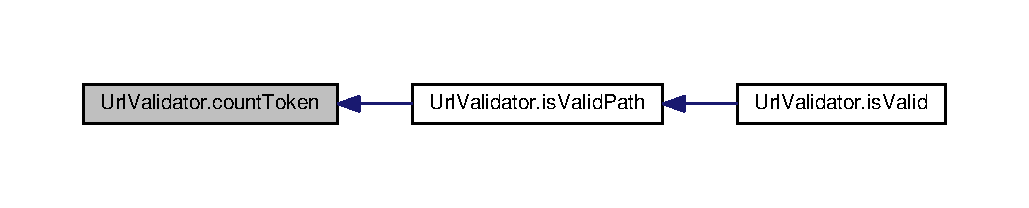
\includegraphics[width=350pt]{classUrlValidator_a80666c758d0f6ef10b8e3039905c28de_icgraph}
\end{center}
\end{figure}


\index{Url\+Validator@{Url\+Validator}!get\+Instance@{get\+Instance}}
\index{get\+Instance@{get\+Instance}!Url\+Validator@{Url\+Validator}}
\subsubsection[{\texorpdfstring{get\+Instance()}{getInstance()}}]{\setlength{\rightskip}{0pt plus 5cm}static {\bf Url\+Validator} Url\+Validator.\+get\+Instance (
\begin{DoxyParamCaption}
{}
\end{DoxyParamCaption}
)\hspace{0.3cm}{\ttfamily [static]}}\hypertarget{classUrlValidator_aeb644e3bf40f37b798b450f15421bfad}{}\label{classUrlValidator_aeb644e3bf40f37b798b450f15421bfad}
Returns the singleton instance of this class with default schemes and options. \begin{DoxyReturn}{Returns}
singleton instance with default schemes and options 
\end{DoxyReturn}
\index{Url\+Validator@{Url\+Validator}!is\+Valid@{is\+Valid}}
\index{is\+Valid@{is\+Valid}!Url\+Validator@{Url\+Validator}}
\subsubsection[{\texorpdfstring{is\+Valid(\+String value)}{isValid(String value)}}]{\setlength{\rightskip}{0pt plus 5cm}boolean Url\+Validator.\+is\+Valid (
\begin{DoxyParamCaption}
\item[{String}]{value}
\end{DoxyParamCaption}
)}\hypertarget{classUrlValidator_aad892796e16502238af06e5de73f1325}{}\label{classUrlValidator_aad892796e16502238af06e5de73f1325}
Checks if a field has a valid url address.


\begin{DoxyParams}{Parameters}
{\em value} & The value validation is being performed on. A {\ttfamily null} value is considered invalid. \\
\hline
\end{DoxyParams}
\begin{DoxyReturn}{Returns}
true if the url is valid. 
\end{DoxyReturn}


Here is the call graph for this function\+:\nopagebreak
\begin{figure}[H]
\begin{center}
\leavevmode
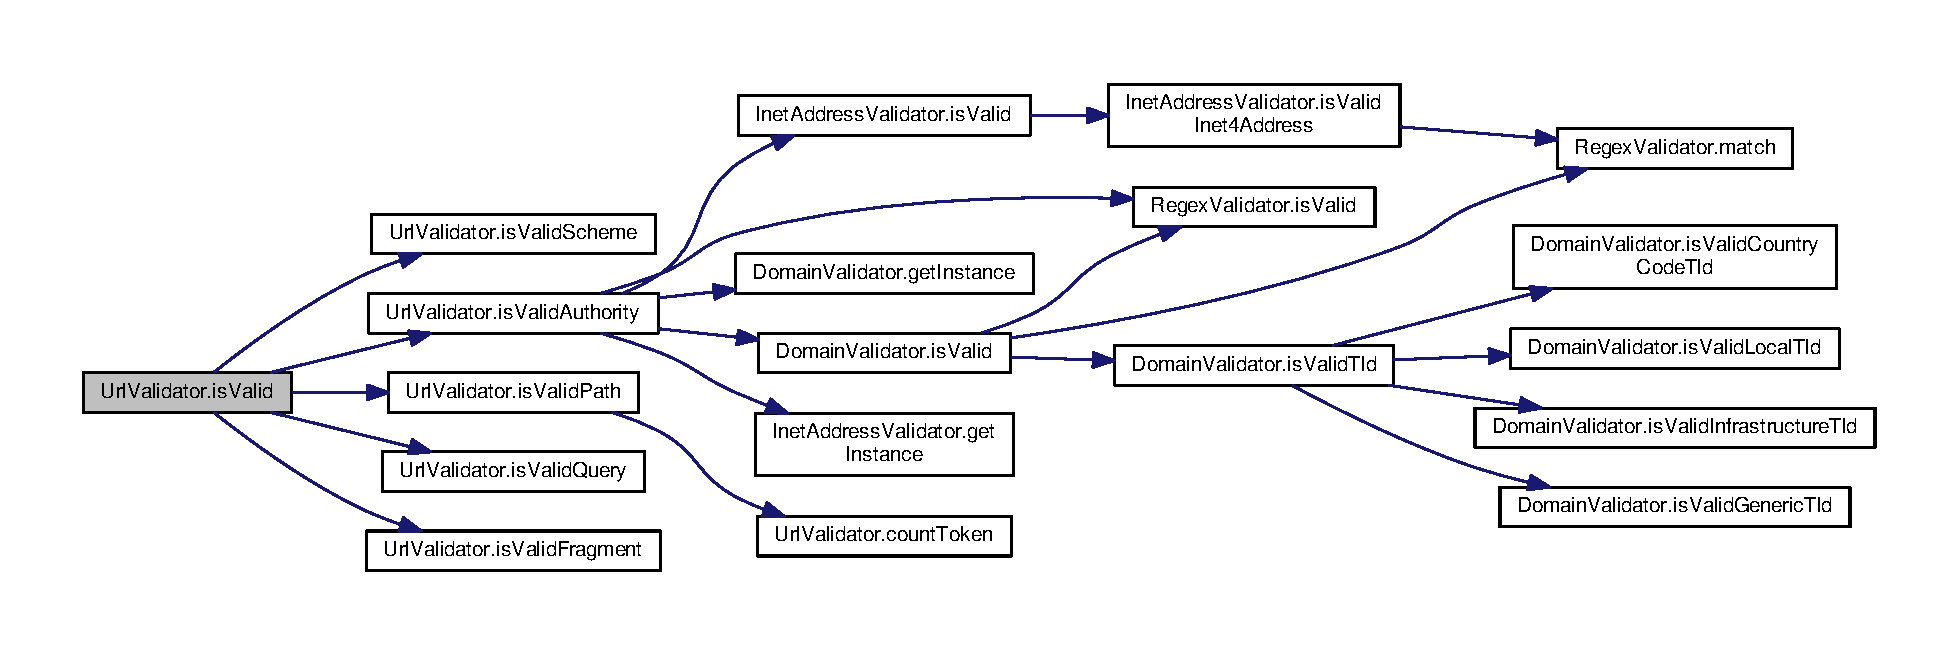
\includegraphics[width=350pt]{classUrlValidator_aad892796e16502238af06e5de73f1325_cgraph}
\end{center}
\end{figure}




Here is the caller graph for this function\+:
\nopagebreak
\begin{figure}[H]
\begin{center}
\leavevmode
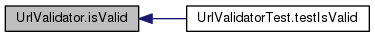
\includegraphics[width=350pt]{classUrlValidator_aad892796e16502238af06e5de73f1325_icgraph}
\end{center}
\end{figure}


\index{Url\+Validator@{Url\+Validator}!is\+Valid\+Authority@{is\+Valid\+Authority}}
\index{is\+Valid\+Authority@{is\+Valid\+Authority}!Url\+Validator@{Url\+Validator}}
\subsubsection[{\texorpdfstring{is\+Valid\+Authority(\+String authority)}{isValidAuthority(String authority)}}]{\setlength{\rightskip}{0pt plus 5cm}boolean Url\+Validator.\+is\+Valid\+Authority (
\begin{DoxyParamCaption}
\item[{String}]{authority}
\end{DoxyParamCaption}
)\hspace{0.3cm}{\ttfamily [protected]}}\hypertarget{classUrlValidator_aeeb764937709a459010e4db60fe70e59}{}\label{classUrlValidator_aeeb764937709a459010e4db60fe70e59}
Returns true if the authority is properly formatted. An authority is the combination of hostname and port. A {\ttfamily null} authority value is considered invalid. 
\begin{DoxyParams}{Parameters}
{\em authority} & Authority value to validate. \\
\hline
\end{DoxyParams}
\begin{DoxyReturn}{Returns}
true if authority (hostname and port) is valid. 
\end{DoxyReturn}


Here is the call graph for this function\+:\nopagebreak
\begin{figure}[H]
\begin{center}
\leavevmode
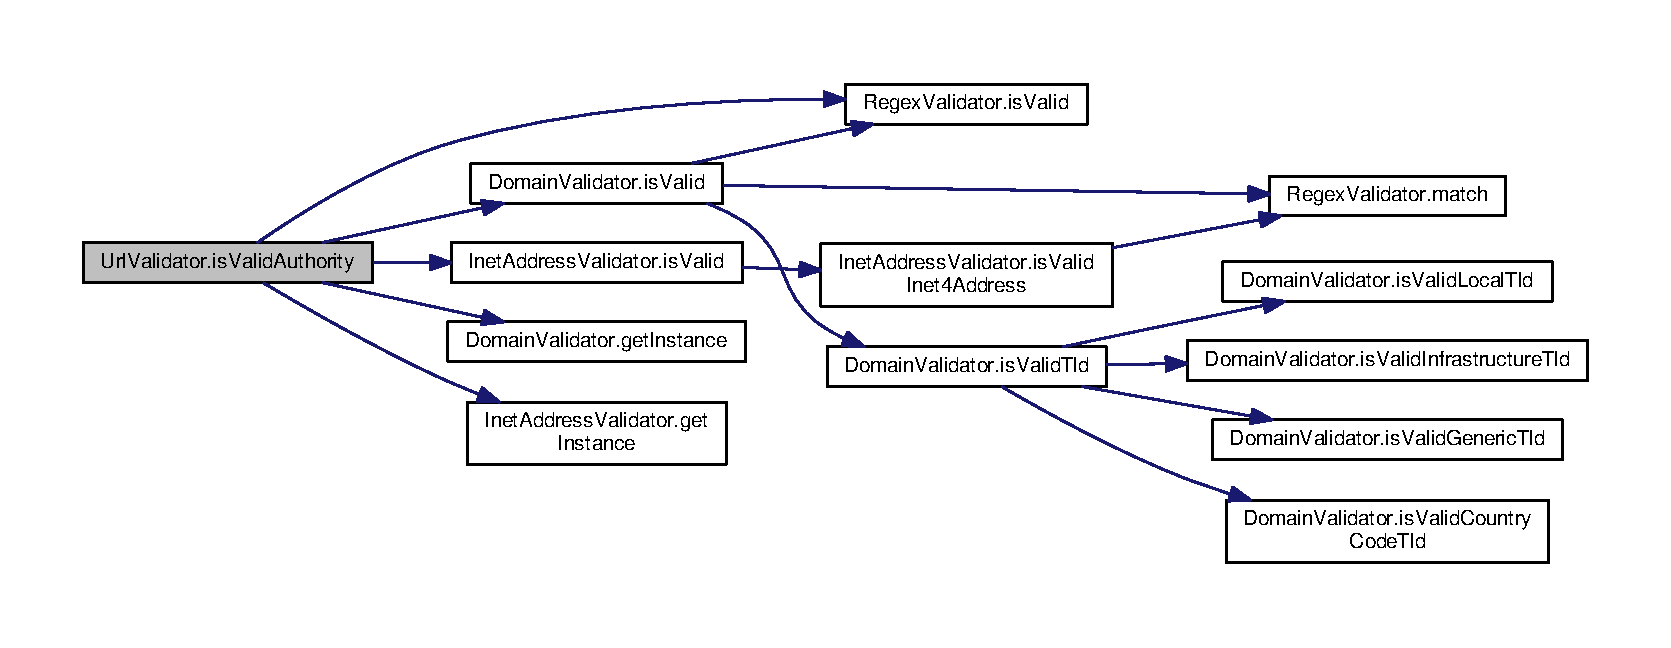
\includegraphics[width=350pt]{classUrlValidator_aeeb764937709a459010e4db60fe70e59_cgraph}
\end{center}
\end{figure}




Here is the caller graph for this function\+:
\nopagebreak
\begin{figure}[H]
\begin{center}
\leavevmode
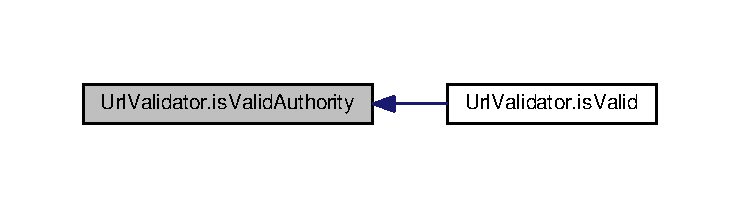
\includegraphics[width=350pt]{classUrlValidator_aeeb764937709a459010e4db60fe70e59_icgraph}
\end{center}
\end{figure}


\index{Url\+Validator@{Url\+Validator}!is\+Valid\+Fragment@{is\+Valid\+Fragment}}
\index{is\+Valid\+Fragment@{is\+Valid\+Fragment}!Url\+Validator@{Url\+Validator}}
\subsubsection[{\texorpdfstring{is\+Valid\+Fragment(\+String fragment)}{isValidFragment(String fragment)}}]{\setlength{\rightskip}{0pt plus 5cm}boolean Url\+Validator.\+is\+Valid\+Fragment (
\begin{DoxyParamCaption}
\item[{String}]{fragment}
\end{DoxyParamCaption}
)\hspace{0.3cm}{\ttfamily [protected]}}\hypertarget{classUrlValidator_ac8fbdf3595973d4a9cebc1bf95c81656}{}\label{classUrlValidator_ac8fbdf3595973d4a9cebc1bf95c81656}
Returns true if the given fragment is null or fragments are allowed. 
\begin{DoxyParams}{Parameters}
{\em fragment} & Fragment value to validate. \\
\hline
\end{DoxyParams}
\begin{DoxyReturn}{Returns}
true if fragment is valid. 
\end{DoxyReturn}


Here is the caller graph for this function\+:
\nopagebreak
\begin{figure}[H]
\begin{center}
\leavevmode
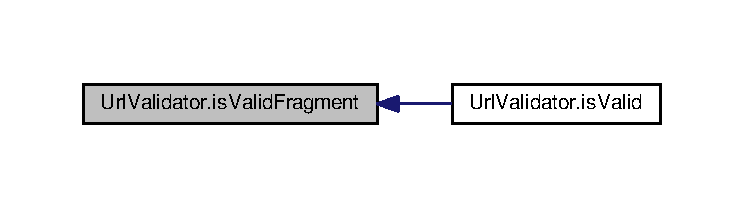
\includegraphics[width=350pt]{classUrlValidator_ac8fbdf3595973d4a9cebc1bf95c81656_icgraph}
\end{center}
\end{figure}


\index{Url\+Validator@{Url\+Validator}!is\+Valid\+Path@{is\+Valid\+Path}}
\index{is\+Valid\+Path@{is\+Valid\+Path}!Url\+Validator@{Url\+Validator}}
\subsubsection[{\texorpdfstring{is\+Valid\+Path(\+String path)}{isValidPath(String path)}}]{\setlength{\rightskip}{0pt plus 5cm}boolean Url\+Validator.\+is\+Valid\+Path (
\begin{DoxyParamCaption}
\item[{String}]{path}
\end{DoxyParamCaption}
)\hspace{0.3cm}{\ttfamily [protected]}}\hypertarget{classUrlValidator_ab0c296806ab80aa80d98e9654d791b05}{}\label{classUrlValidator_ab0c296806ab80aa80d98e9654d791b05}
Returns true if the path is valid. A {\ttfamily null} value is considered invalid. 
\begin{DoxyParams}{Parameters}
{\em path} & Path value to validate. \\
\hline
\end{DoxyParams}
\begin{DoxyReturn}{Returns}
true if path is valid. 
\end{DoxyReturn}


Here is the call graph for this function\+:\nopagebreak
\begin{figure}[H]
\begin{center}
\leavevmode
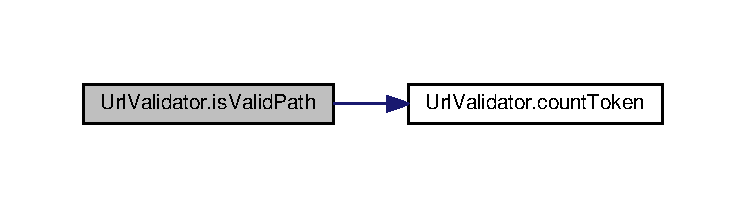
\includegraphics[width=350pt]{classUrlValidator_ab0c296806ab80aa80d98e9654d791b05_cgraph}
\end{center}
\end{figure}




Here is the caller graph for this function\+:
\nopagebreak
\begin{figure}[H]
\begin{center}
\leavevmode
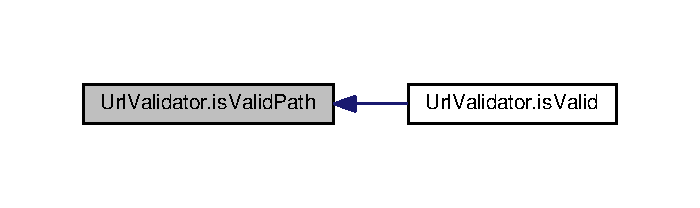
\includegraphics[width=350pt]{classUrlValidator_ab0c296806ab80aa80d98e9654d791b05_icgraph}
\end{center}
\end{figure}


\index{Url\+Validator@{Url\+Validator}!is\+Valid\+Query@{is\+Valid\+Query}}
\index{is\+Valid\+Query@{is\+Valid\+Query}!Url\+Validator@{Url\+Validator}}
\subsubsection[{\texorpdfstring{is\+Valid\+Query(\+String query)}{isValidQuery(String query)}}]{\setlength{\rightskip}{0pt plus 5cm}boolean Url\+Validator.\+is\+Valid\+Query (
\begin{DoxyParamCaption}
\item[{String}]{query}
\end{DoxyParamCaption}
)\hspace{0.3cm}{\ttfamily [protected]}}\hypertarget{classUrlValidator_a509b2d886b639de2b1c55e6e3707ba5f}{}\label{classUrlValidator_a509b2d886b639de2b1c55e6e3707ba5f}
Returns true if the query is null or it\textquotesingle{}s a properly formatted query string. 
\begin{DoxyParams}{Parameters}
{\em query} & Query value to validate. \\
\hline
\end{DoxyParams}
\begin{DoxyReturn}{Returns}
true if query is valid. 
\end{DoxyReturn}


Here is the caller graph for this function\+:
\nopagebreak
\begin{figure}[H]
\begin{center}
\leavevmode
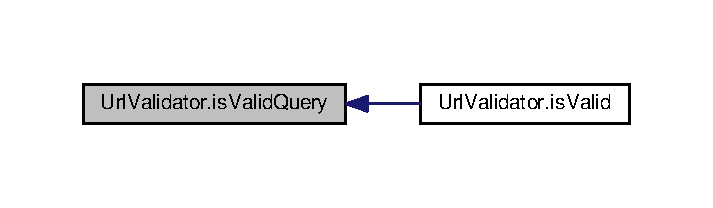
\includegraphics[width=350pt]{classUrlValidator_a509b2d886b639de2b1c55e6e3707ba5f_icgraph}
\end{center}
\end{figure}


\index{Url\+Validator@{Url\+Validator}!is\+Valid\+Scheme@{is\+Valid\+Scheme}}
\index{is\+Valid\+Scheme@{is\+Valid\+Scheme}!Url\+Validator@{Url\+Validator}}
\subsubsection[{\texorpdfstring{is\+Valid\+Scheme(\+String scheme)}{isValidScheme(String scheme)}}]{\setlength{\rightskip}{0pt plus 5cm}boolean Url\+Validator.\+is\+Valid\+Scheme (
\begin{DoxyParamCaption}
\item[{String}]{scheme}
\end{DoxyParamCaption}
)\hspace{0.3cm}{\ttfamily [protected]}}\hypertarget{classUrlValidator_a9a598e3ca397702e2a36033965993fc7}{}\label{classUrlValidator_a9a598e3ca397702e2a36033965993fc7}
Validate scheme. If schemes\mbox{[}\mbox{]} was initialized to a non null, then only those scheme\textquotesingle{}s are allowed. Note this is slightly different than for the constructor. 
\begin{DoxyParams}{Parameters}
{\em scheme} & The scheme to validate. A {\ttfamily null} value is considered invalid. \\
\hline
\end{DoxyParams}
\begin{DoxyReturn}{Returns}
true if valid. 
\end{DoxyReturn}


Here is the caller graph for this function\+:
\nopagebreak
\begin{figure}[H]
\begin{center}
\leavevmode
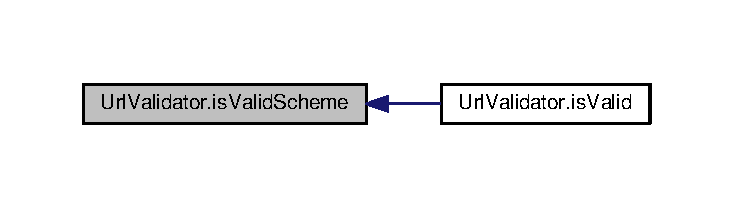
\includegraphics[width=350pt]{classUrlValidator_a9a598e3ca397702e2a36033965993fc7_icgraph}
\end{center}
\end{figure}




\subsection{Member Data Documentation}
\index{Url\+Validator@{Url\+Validator}!A\+L\+L\+O\+W\+\_\+2\+\_\+\+S\+L\+A\+S\+H\+ES@{A\+L\+L\+O\+W\+\_\+2\+\_\+\+S\+L\+A\+S\+H\+ES}}
\index{A\+L\+L\+O\+W\+\_\+2\+\_\+\+S\+L\+A\+S\+H\+ES@{A\+L\+L\+O\+W\+\_\+2\+\_\+\+S\+L\+A\+S\+H\+ES}!Url\+Validator@{Url\+Validator}}
\subsubsection[{\texorpdfstring{A\+L\+L\+O\+W\+\_\+2\+\_\+\+S\+L\+A\+S\+H\+ES}{ALLOW_2_SLASHES}}]{\setlength{\rightskip}{0pt plus 5cm}final long Url\+Validator.\+A\+L\+L\+O\+W\+\_\+2\+\_\+\+S\+L\+A\+S\+H\+ES = 1 $<$$<$ 1\hspace{0.3cm}{\ttfamily [static]}}\hypertarget{classUrlValidator_a2a0966f94123825fcef6816a5d684ed2}{}\label{classUrlValidator_a2a0966f94123825fcef6816a5d684ed2}
Allow two slashes in the path component of the U\+RL. \index{Url\+Validator@{Url\+Validator}!A\+L\+L\+O\+W\+\_\+\+A\+L\+L\+\_\+\+S\+C\+H\+E\+M\+ES@{A\+L\+L\+O\+W\+\_\+\+A\+L\+L\+\_\+\+S\+C\+H\+E\+M\+ES}}
\index{A\+L\+L\+O\+W\+\_\+\+A\+L\+L\+\_\+\+S\+C\+H\+E\+M\+ES@{A\+L\+L\+O\+W\+\_\+\+A\+L\+L\+\_\+\+S\+C\+H\+E\+M\+ES}!Url\+Validator@{Url\+Validator}}
\subsubsection[{\texorpdfstring{A\+L\+L\+O\+W\+\_\+\+A\+L\+L\+\_\+\+S\+C\+H\+E\+M\+ES}{ALLOW_ALL_SCHEMES}}]{\setlength{\rightskip}{0pt plus 5cm}final long Url\+Validator.\+A\+L\+L\+O\+W\+\_\+\+A\+L\+L\+\_\+\+S\+C\+H\+E\+M\+ES = 1 $<$$<$ 0\hspace{0.3cm}{\ttfamily [static]}}\hypertarget{classUrlValidator_a1cd6766c458c99db9d98b585417a9623}{}\label{classUrlValidator_a1cd6766c458c99db9d98b585417a9623}
Allows all validly formatted schemes to pass validation instead of supplying a set of valid schemes. \index{Url\+Validator@{Url\+Validator}!A\+L\+L\+O\+W\+\_\+\+L\+O\+C\+A\+L\+\_\+\+U\+R\+LS@{A\+L\+L\+O\+W\+\_\+\+L\+O\+C\+A\+L\+\_\+\+U\+R\+LS}}
\index{A\+L\+L\+O\+W\+\_\+\+L\+O\+C\+A\+L\+\_\+\+U\+R\+LS@{A\+L\+L\+O\+W\+\_\+\+L\+O\+C\+A\+L\+\_\+\+U\+R\+LS}!Url\+Validator@{Url\+Validator}}
\subsubsection[{\texorpdfstring{A\+L\+L\+O\+W\+\_\+\+L\+O\+C\+A\+L\+\_\+\+U\+R\+LS}{ALLOW_LOCAL_URLS}}]{\setlength{\rightskip}{0pt plus 5cm}final long Url\+Validator.\+A\+L\+L\+O\+W\+\_\+\+L\+O\+C\+A\+L\+\_\+\+U\+R\+LS = 1 $<$$<$ 3\hspace{0.3cm}{\ttfamily [static]}}\hypertarget{classUrlValidator_a8614b7832fddf98bff7ddfb5dfdbff75}{}\label{classUrlValidator_a8614b7832fddf98bff7ddfb5dfdbff75}
Allow local U\+R\+Ls, such as \href{http://localhost/}{\tt http\+://localhost/} or \href{http://machine/}{\tt http\+://machine/} . This enables a broad-\/brush check, for complex local machine name validation requirements you should create your validator with a \hyperlink{classRegexValidator}{Regex\+Validator} instead (\hyperlink{classUrlValidator_a4dcb6938b73df2c093739f03ac6ed52d}{Url\+Validator(\+Regex\+Validator, long)}) \index{Url\+Validator@{Url\+Validator}!N\+O\+\_\+\+F\+R\+A\+G\+M\+E\+N\+TS@{N\+O\+\_\+\+F\+R\+A\+G\+M\+E\+N\+TS}}
\index{N\+O\+\_\+\+F\+R\+A\+G\+M\+E\+N\+TS@{N\+O\+\_\+\+F\+R\+A\+G\+M\+E\+N\+TS}!Url\+Validator@{Url\+Validator}}
\subsubsection[{\texorpdfstring{N\+O\+\_\+\+F\+R\+A\+G\+M\+E\+N\+TS}{NO_FRAGMENTS}}]{\setlength{\rightskip}{0pt plus 5cm}final long Url\+Validator.\+N\+O\+\_\+\+F\+R\+A\+G\+M\+E\+N\+TS = 1 $<$$<$ 2\hspace{0.3cm}{\ttfamily [static]}}\hypertarget{classUrlValidator_a9f6b028f570818955c807cfe97e29641}{}\label{classUrlValidator_a9f6b028f570818955c807cfe97e29641}
Enabling this options disallows any U\+RL fragments. 

The documentation for this class was generated from the following file\+:\begin{DoxyCompactItemize}
\item 
src/Url\+Validator.\+java\end{DoxyCompactItemize}

\hypertarget{classUrlValidatorTest}{}\section{Url\+Validator\+Test Class Reference}
\label{classUrlValidatorTest}\index{Url\+Validator\+Test@{Url\+Validator\+Test}}


Inheritance diagram for Url\+Validator\+Test\+:
\nopagebreak
\begin{figure}[H]
\begin{center}
\leavevmode
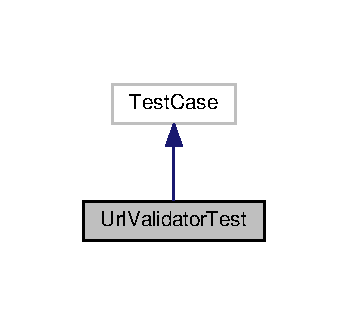
\includegraphics[width=167pt]{classUrlValidatorTest__inherit__graph}
\end{center}
\end{figure}


Collaboration diagram for Url\+Validator\+Test\+:
\nopagebreak
\begin{figure}[H]
\begin{center}
\leavevmode
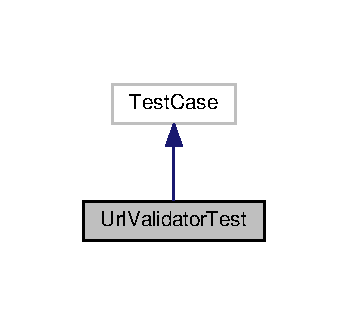
\includegraphics[width=167pt]{classUrlValidatorTest__coll__graph}
\end{center}
\end{figure}
\subsection*{Public Member Functions}
\begin{DoxyCompactItemize}
\item 
{\bfseries Url\+Validator\+Test} (String test\+Name)\hypertarget{classUrlValidatorTest_a4796e3be2cbb63250e9bf3c6a96c84eb}{}\label{classUrlValidatorTest_a4796e3be2cbb63250e9bf3c6a96c84eb}

\item 
void {\bfseries test\+Manual\+Test} ()\hypertarget{classUrlValidatorTest_a41ceee2038da5ca23bbec7c9270d5009}{}\label{classUrlValidatorTest_a41ceee2038da5ca23bbec7c9270d5009}

\item 
void {\bfseries test\+Your\+First\+Partition} ()\hypertarget{classUrlValidatorTest_aa26e45c1e214b9c3daab746dbb788315}{}\label{classUrlValidatorTest_aa26e45c1e214b9c3daab746dbb788315}

\item 
void {\bfseries test\+Your\+Second\+Partition} ()\hypertarget{classUrlValidatorTest_a5a8fa86d6116d95574b69a739f839fd3}{}\label{classUrlValidatorTest_a5a8fa86d6116d95574b69a739f839fd3}

\item 
void {\bfseries test\+Is\+Valid} ()\hypertarget{classUrlValidatorTest_a46c190729e25d1f0a4ab52ec51f0397e}{}\label{classUrlValidatorTest_a46c190729e25d1f0a4ab52ec51f0397e}

\item 
void {\bfseries test\+Any\+Other\+Unit\+Test} ()\hypertarget{classUrlValidatorTest_a6abe80d9902e0d05e0298c9f149f060f}{}\label{classUrlValidatorTest_a6abe80d9902e0d05e0298c9f149f060f}

\end{DoxyCompactItemize}


\subsection{Detailed Description}
Performs Validation Test for url validations.

\begin{DoxyVersion}{Version}

\end{DoxyVersion}
\begin{DoxyParagraph}{Revision}
1128446 
\end{DoxyParagraph}
\begin{DoxyParagraph}{Date}
2011-\/05-\/27 13\+:29\+:27 -\/0700 (Fri, 27 May 2011) 
\end{DoxyParagraph}


The documentation for this class was generated from the following file\+:\begin{DoxyCompactItemize}
\item 
src/Url\+Validator\+Test.\+java\end{DoxyCompactItemize}

%--- End generated contents ---

% Index
\backmatter
\newpage
\phantomsection
\clearemptydoublepage
\addcontentsline{toc}{chapter}{Index}
\printindex

\end{document}
